\documentclass[a4paper,12pt]{article}
\usepackage[utf8]{vntex}
\usepackage[english,vietnamese]{babel}
\usepackage{amsmath,amssymb,amsthm,latexsym}
\usepackage{geometry}
\geometry{a4paper, left=22mm, top=22mm, right=18mm, bottom=22mm}

\usepackage{booktabs}
\usepackage{tabularx}
\usepackage{array}
\usepackage{multirow}
\usepackage{makecell}
\usepackage{hhline}
\usepackage{adjustbox}
\usepackage[skip=6pt]{caption}
\usepackage{enumitem}
\usepackage{lastpage}
\usepackage{fancyhdr}
\usepackage{multicol}
\usepackage{rotating}
\usepackage{setspace}
\usepackage{placeins}
\usepackage{float}

\usepackage{graphicx}
\usepackage{epsfig}
\usepackage{tikz}
\usetikzlibrary{arrows.meta,backgrounds,positioning,shapes.geometric,automata,calc,fit}
\usepackage[framemethod=tikz]{mdframed}
\usepackage{tcolorbox}
\tcbuselibrary{skins,breakable}

\usepackage{algorithm}
\usepackage{algpseudocode}
\usepackage{listings}

\usepackage{xcolor}
\setlength{\columnseprule}{1pt}
\def\columnseprulecolor{\color{black}}
\definecolor{codegreen}{rgb}{0,0.45,0}
\definecolor{codegray}{rgb}{0.45,0.45,0.45}
\definecolor{codepurple}{rgb}{0.45,0,0.6}
\definecolor{backcolour}{rgb}{0.97,0.97,0.97}
\definecolor{keywordblue}{rgb}{0.1,0.2,0.55}
\definecolor{bordergray}{rgb}{0.75,0.75,0.75}

% --- Giữ đủ 3 tên màu cho sơ đồ TikZ ở de_bai.tex & module3.tex (tông trầm, đồng bộ) ---
\definecolor{navyaccent}{RGB}{38,50,66}
\definecolor{tealaccent}{RGB}{52,84,84}
\definecolor{amberaccent}{RGB}{105,82,58}

% --- Cho phép dàn dòng linh hoạt, hạn chế tràn lề ---
\setlength{\emergencystretch}{2em}

% --- Cột bảng tự xuống dòng khớp chuẩn \textwidth ---
\newcolumntype{L}{>{\raggedright\arraybackslash}X}
\newcolumntype{C}{>{\centering\arraybackslash}X}
\newcolumntype{R}{>{\raggedleft\arraybackslash}X}

% --- Định dạng Caption bảng đặt phía trên giống mẫu học thuật ---
\captionsetup[table]{
    position=top,
    justification=centering,
    labelfont=normalfont,
    textfont=normalfont,
    skip=6pt
}
\captionsetup[figure]{
    position=bottom,
    justification=centering,
    skip=6pt
}

\lstset{
    language=Python,
    backgroundcolor=\color{backcolour},
    frame=tb,
    framerule=0.5pt,
    rulecolor=\color{bordergray},
    basicstyle=\ttfamily\footnotesize,
    keywordstyle=\color{keywordblue}\bfseries,
    commentstyle=\color{codegray}\itshape,
    numberstyle=\tiny\color{codegray},
    numbers=left,
    stepnumber=1,
    breaklines=true,
    breakatwhitespace=false,
    linewidth=\linewidth,
    xleftmargin=12pt,
    tabsize=4,
    showstringspaces=false
}

% --- Khung cơ sở lý thuyết siêu tối giản: nền trắng, chỉ 2 đường kẻ ngang đồng bộ bảng ---
\newtcolorbox{theorybox}[2][]{
    enhanced,
    breakable,
    sharp corners,
    width=\linewidth,
    boxsep=0pt,
    left=0pt, right=0pt, top=5pt, bottom=5pt,
    toptitle=4pt, bottomtitle=4pt,
    colback=white,
    colbacktitle=white,
    colframe=black!85,
    coltitle=black,
    fonttitle=\bfseries\small,
    boxrule=0pt,
    toprule=0.8pt,
    bottomrule=0.8pt,
    titlerule=0.4pt,
    titlerule style={black!35},
    before skip=10pt, after skip=10pt,
    title={#2},
    #1
}

% --- Khung ghi chú tối giản: nền trắng, vạch dọc mảnh bên trái ---
\newtcolorbox{notebox}[2][]{
    enhanced,
    breakable,
    sharp corners,
    width=\linewidth,
    boxsep=0pt,
    left=8pt, right=0pt, top=3pt, bottom=3pt,
    toptitle=2pt, bottomtitle=2pt,
    colback=white,
    colbacktitle=white,
    colframe=white,
    coltitle=black!85,
    fonttitle=\bfseries\small,
    boxrule=0pt,
    titlerule=0pt,
    borderline west={1.2pt}{0pt}{black!45},
    before skip=8pt, after skip=8pt,
    title={#2},
    #1
}

% Bỏ dấu % dòng dưới nếu muốn công thức toán màu xanh dương:
% \everymath{\color{blue}}

\usepackage{hyperref}
\hypersetup{
    urlcolor=black,
    linkcolor=black,
    citecolor=black,
    colorlinks=true
}

% --- Header & Footer ---
\setlength{\headheight}{36pt}
\pagestyle{fancy}
\fancyhead{}
\fancyhead[L]{
  \begin{tabular}{@{}rl@{}}
    \begin{picture}(25,15)(0,0)
      \put(0,-8){
\includegraphics[width=8mm, height=8mm]{hcmut.png}}
    \end{picture}&
    \begin{tabular}{@{}l@{}}
      {\ttfamily University of Technology}\\
      {\ttfamily Faculty of Computer Science and Engineering}
    \end{tabular}
  \end{tabular}
}
\fancyhead[R]{\scriptsize \ttfamily CO2011-261-A01-2551896}
\fancyfoot{}
\fancyfoot[L]{\scriptsize \ttfamily Mathematical Modeling (CO2011) Assignment, Semester 261}
\fancyfoot[R]{\scriptsize \ttfamily Page {\thepage}/\pageref{LastPage}}
\renewcommand{\headrulewidth}{0.3pt}
\renewcommand{\footrulewidth}{0.3pt}

% --- Cấu hình cấp mục & khoảng cách gọn cho giới hạn <= 20 trang ---
\setcounter{secnumdepth}{4}
\setcounter{tocdepth}{2}
\setlist[itemize]{itemsep=2pt, topsep=3pt, parsep=0pt}
\setlist[enumerate]{itemsep=2pt, topsep=3pt, parsep=0pt}
\makeatletter
\newcounter{subsubsubsection}[subsubsection]
\renewcommand\thesubsubsubsection{\thesubsubsection.\@alph\c@subsubsubsection}
\newcommand\subsubsubsection{\@startsection{subsubsubsection}{4}{\z@}%
                                     {-3.25ex\@plus -1ex \@minus -.2ex}%
                                     {1.5ex \@plus .2ex}%
                                     {\normalfont\normalsize\bfseries}}
\newcommand*\l@subsubsubsection{\@dottedtocline{3}{10.0em}{4.1em}}
\newcommand*{\subsubsubsectionmark}[1]{}
\makeatother

\begin{document}

% ==================== TRANG BÌA ====================
\pagenumbering{Alph}
\newgeometry{margin=20mm}
\begin{titlepage}
\begin{tikzpicture}[remember picture, overlay]
    \draw[line width = 2pt, color = black]
        ([xshift=15mm, yshift=-15mm]current page.north west)
        rectangle
        ([xshift=-15mm, yshift=15mm]current page.south east);

    \draw[line width = 0.8pt, color = black]
        ([xshift=17.5mm, yshift=-17.5mm]current page.north west)
        rectangle
        ([xshift=-17.5mm, yshift=17.5mm]current page.south east);
\end{tikzpicture}

\begin{center}
    {\Large
    Vietnam National University, Ho Chi Minh City \\
    Ho Chi Minh City University of Technology (HCMUT) \\
    Faculty of Computer Science and Engineering\par}
\end{center}

\vspace{0.8cm}

\begin{figure}[h!]
    \centering
    
\includegraphics[width=3.8cm]{hcmut.png}
\end{figure}

\vspace{0.6cm}

\begin{center}
\begin{minipage}{0.95\textwidth}
    \centering
    {\Large\bfseries MATHEMATICAL MODELING (CO2011)\par}
    \vspace{8pt}
    \rule{\linewidth}{0.6pt}
    \vspace{12pt}

    {\large\bfseries Semester-long Integrated Assignment\par}
    \vspace{10pt}

    \resizebox{0.96\linewidth}{!}{\bfseries INVIGILATOR ASSIGNMENT PROBLEM}\par
    \vspace{10pt}

    {\small\textit{Logic $\Rightarrow$ Linear \& Integer Programming $\Rightarrow$ Automata $\Rightarrow$ Dynamical Systems $\Rightarrow$ Web App}\par}
    \vspace{10pt}
    \rule{\linewidth}{0.6pt}
\end{minipage}
\end{center}

\vspace{1.0cm}

\begin{center}
\begin{tabular}{r l l}
    \textbf{Instructor(s):} & Phạm An Vinh, CSE-HCMUT & \\
    \textbf{Class:}         & A01 & \\
    \textbf{Team ID:}       & \texttt{CO2011-261-A01-2551896} & \\
    \textbf{Team Seed:}     & \texttt{1358677812} \; ($\lambda = (0.84, 1.90, 1.97)$) & \\
    \textbf{Students:}      & Võ Nguyễn Vĩ Nguyên    & - 2551913 \\
                            & Chu Ngọc Phúc Thành    & - 2551922 \\
                            & Đinh Hoàng Quang Vinh  & - 2551931 \\
                            & Đặng Nguyễn Thiên Phúc & - 2551919 \\
                            & Nguyễn Quốc Hùng       & - 2551896 \\
\end{tabular}
\end{center}

\vfill

\begin{center}
    {\footnotesize Ho Chi Minh City, Semester 261 (2026--2027)}
\end{center}
\end{titlepage}
\restoregeometry

% ========================================
\pagenumbering{roman}
\thispagestyle{fancy}
\tableofcontents
\newpage

% ==================== NỘI DUNG CHÍNH (<= 20 TRANG) ====================
\pagenumbering{arabic}
\setcounter{page}{1}

\section{Tổng quan Bài toán và Kiến trúc Hệ thống}
\label{sec:overview}

\subsection{Bối cảnh và Phát biểu Bài toán Phân công Cán bộ Coi thi (IAP)}
Mỗi học kỳ, Khoa Khoa học và Kỹ thuật Máy tính (CSE--HCMUT) phải tổ chức hàng trăm lượt coi thi tại hai cơ sở cách xa nhau: Cơ sở 1 (Lý Thường Kiệt -- \texttt{CS1}) và Cơ sở 2 (Dĩ An -- \texttt{CS2}). Bài toán \textbf{Invigilator Assignment Problem (IAP)} yêu cầu phân công đủ số lượng cán bộ coi thi cho từng ca thi trong khi vừa bảo đảm tuyệt đối các quy định bắt buộc (\textit{hard constraints}: đủ định ngạch, không phân công khi bận, không trùng giờ), vừa tối ưu sự công bằng tải trọng và các ràng buộc mềm (\textit{soft constraints}: nguyện vọng cơ sở, giới hạn mệt mỏi, hạn chế di chuyển liên cơ sở) \cite{hanum2015,burke2004}. Về bản chất tổ hợp, IAP là một bài toán thỏa mãn ràng buộc và tối ưu rời rạc thuộc lớp \textbf{NP-hard} \cite{nemhauser1999}.

Bộ dữ liệu thực tế đã ẩn danh (\texttt{data/input.csv}) ghi nhận lịch coi thi gốc (\textit{Baseline}) gồm các thông số:
\begin{itemize}
    \item \textbf{Tập cán bộ ($N = 73$):} Gồm $73$ mã cán bộ (\texttt{CB001}--\texttt{CB073}). Theo thiết kế thống nhất của toàn đồ án (\texttt{m1\_\allowbreak logic/\allowbreak data\_\allowbreak loader.py}), toàn bộ vai trò (\texttt{CBCT}, \texttt{Thư ký}, \texttt{Trưởng HĐ}) được gộp chung thành lực lượng coi thi đồng nhất, không áp đặt ràng buộc phân hạng riêng.
    \item \textbf{Tập ca thi ($M = 83$) trên $65$ mã khung giờ:} Mỗi ca thi $j \in J$ là một cặp duy nhất $(\text{MS Ca thi}, \text{Cơ sở})$, gồm $45$ ca tại \texttt{CS1} và $38$ ca tại \texttt{CS2}, diễn ra trong $23$ ngày thi thuộc khung lịch liên tục $T = 27$ ngày từ 18/05/2026 đến 13/06/2026.
    \item \textbf{Tổng định ngạch và lịch gốc:} Tổng nhu cầu nhân sự toàn kỳ là $\sum_{j \in J} r_j = 769$ lượt phân công (ca lớn nhất cần $32$ cán bộ), với $18$ cặp ca thi trùng giờ (toàn bộ là cùng mã ca diễn ra đồng thời tại \texttt{CS1} và \texttt{CS2}; các ca tiếp giáp đầu--cuối như 07:00--09:30 và 09:30--12:00 không tính là trùng). Lịch gốc thủ công (\texttt{Baseline}) mất cân bằng nghiêm trọng với tải đỉnh $\text{max\_load} = 19$, $\text{min\_load} = 3$ ($\text{spread} = 16$, $L_1 = 115{,}397$).
\end{itemize}

\subsection{Tính Tái lập theo Seed và Các Giả định Mô phỏng}
Toàn bộ kết quả thực nghiệm của nhóm được định danh duy nhất bằng \texttt{Team ID = CO2011-\allowbreak 261-\allowbreak A01-\allowbreak 2551896}. Hàm băm BLAKE2 trong \texttt{tools/\allowbreak make\_\allowbreak seed.py} sinh tất định mã seed \texttt{1358677812} (\texttt{data/seed.txt}) và bộ ba trọng số phạt mềm $\lambda = (0{,}84;\, 1{,}90;\, 1{,}97)$. Mọi bảng số liệu và hình ảnh trong báo cáo được tái tạo tự động bằng lệnh duy nhất: \texttt{python run\_all.py --seed \$(cat data/seed.txt)}.

Tuân thủ nguyên tắc \textit{``fit, don't fabricate''}, mọi cấu phần dữ liệu thực không cung cấp trực tiếp đều được mô phỏng có kiểm soát và công bố minh bạch trong Bảng~\ref{tab:assumptions}.

\begin{table}[htbp]
\centering
\caption{Tổng hợp các giả định mô phỏng từ dữ liệu thực với \texttt{seed = 1358677812}.}
\label{tab:assumptions}
\small
\setlength{\tabcolsep}{5pt}
\renewcommand{\arraystretch}{1.22}
\begin{tabularx}{\textwidth}{@{} >{\raggedright\arraybackslash}p{3.1cm} >{\raggedright\arraybackslash}p{5.6cm} L @{}}
\toprule
\textbf{Thành phần giả định} & \textbf{Quy tắc sinh / hiệu chuẩn} & \textbf{Ý nghĩa và giới hạn thực tế} \\
\midrule
Lịch khả dụng $A$ (Module 1--2) & Giữ nguyên $769$ cặp $(\text{người}, \text{mã ca})$ từng coi ở Baseline; mỗi cặp chưa xuất hiện được mở với xác suất $p = 0{,}30$ dùng \texttt{Random(seed)} (chia sẻ theo mã ca giữa hai cơ sở). & Tạo $1{,}182$ cặp ca mới $\Rightarrow |A| = 2{,}593$ cặp $(\text{người}, \text{ca})$ khả dụng trên $6{,}059$. Sự vắng mặt trong lịch gốc không đồng nghĩa nghỉ phép thực tế. \\
Nguyện vọng cơ sở (Module 2) & $P(\text{BAL}) = 1/3$; $2/3$ còn lại chia theo tỷ lệ làm việc lịch sử tại \texttt{CS1}/\texttt{CS2} của từng người (\texttt{simulated\_\allowbreak preferences.csv}). & Thu được $16$ \texttt{CS1}, $29$ \texttt{CS2}, $28$ \texttt{BAL}. Trọng số phạt: $\lambda_{\text{LOC}} = 0{,}84$, $\lambda_{\text{FAT}} = 1{,}90$, $\lambda_{\text{TRV}} = 1{,}97$. \\
Ca tối \texttt{N} và ngày 2 ca (Module 3) & Khung giờ 18g15 được gán nhãn ca tối \texttt{N}; $169$ cặp $(\text{người}, \text{ngày})$ làm $2$ ca khác buổi được nén về $1$ ký hiệu theo ưu tiên $\texttt{N} > \texttt{A} > \texttt{M}$. & Bảo toàn bảng chữ cái $\Sigma = \{\texttt{M}, \texttt{A}, \texttt{N}, \texttt{-}\}$; hệ quả là $168/169$ ngày hai ca (\texttt{M+A}) được ghi nhận là \texttt{A} khi kiểm tra R4. \\
Proxy mệt mỏi $F_n$ (Module 4) & Hồi quy OLS trễ bậc 1 trên suất tuần lịch sử cho $a = 0{,}270634$ ($R^2 = 0{,}0619$); đặt $r = 0$ và chuẩn hóa $b = 1 - a = 0{,}729366$. & $F_n$ là đại lượng đại diện theo đơn vị tải tuần (\textit{workload proxy}), không phải chỉ số sinh lý hay giới hạn y tế. \\
\bottomrule
\end{tabularx}
\end{table}

\subsection{Kiến trúc Tích hợp Bốn Học phần Lý thuyết CO2011}
Đồ án kết nối bốn học phần lý thuyết của môn \textit{Mô hình hóa Toán học (CO2011)} trên cùng một bài toán thực tế xuyên suốt (Hình~\ref{fig:pipeline_arch}), đồng thời ánh xạ chặt chẽ từng khái niệm trong bộ slide giảng dạy (Bảng~\ref{tab:slide_mapping}).

\begin{figure}[htbp]
\centering
\begin{adjustbox}{max width=\textwidth}
\begin{tikzpicture}[
    node distance=0.55cm and 0.45cm,
    box/.style={rectangle, draw=black!80, fill=white, line width=0.6pt, text width=2.45cm, minimum height=1.25cm, align=center, font=\scriptsize},
    arr/.style={->, >=Stealth, semithick, color=black!80}
]
\node[box, fill=black!4] (data) {\textbf{Dữ liệu \& Seed}\\ $N=73, M=83$\\ $|A|=2{,}593$};
\node[box, right=of data] (m1) {\textbf{Module 1: Logic}\\ FOL $\to$ CNF\\ SAT \& UNSAT Core};
\node[box, right=of m1] (m2) {\textbf{Module 2: ILP}\\ Tối ưu 2 giai đoạn\\ $t^* = 11$, $L_1$, Soft};
\node[box, right=of m2] (m3) {\textbf{Module 3: DFA}\\ R1--R3 (15 tr.thái)\\ Flow ILP ($T=27$)};
\node[box, right=of m3] (m4) {\textbf{Module 4: Động lực}\\ Hướng B: $F_{n+1}$\\ Ổn định \& Ngưỡng $H$};

\draw[arr] (data) -- (m1);
\draw[arr] (m1) -- node[above, font=\tiny]{Bridge} (m2);
\draw[arr] (m2) -- node[above, font=\tiny]{$x_{ij}$} (m3);
\draw[arr] (m3) -- node[above, font=\tiny]{$\ell, L_k$} (m4);

\node[rectangle, draw=black!80, fill=black!3, line width=0.6pt, below=0.55cm of m3, text width=11.8cm, align=center, font=\scriptsize, minimum height=0.75cm] (m5) {\textbf{Module 5: Ứng dụng Web Streamlit (\texttt{app/app.py})} --- Tích hợp kiểm tra SAT, lập lịch ILP, kiểm định DFA R1--R3 và mô phỏng quỹ đạo công bằng trên cùng giao diện tương tác};

\draw[arr] (m1.south) |- (m5.west);
\draw[arr] (m2.south) -- (m2.south |- m5.north);
\draw[arr] (m3.south) -- (m5.north);
\draw[arr] (m4.south) |- (m5.east);
\end{tikzpicture}
\end{adjustbox}
\caption{Kiến trúc luồng dữ liệu tích hợp năm module của hệ thống IAP.}
\label{fig:pipeline_arch}
\end{figure}

\begin{table}[htbp]
\centering
\caption{Ánh xạ trực tiếp từ giáo trình CO2011 sang bốn module thuật toán.}
\label{tab:slide_mapping}
\small
\setlength{\tabcolsep}{5pt}
\renewcommand{\arraystretch}{1.22}
\begin{tabularx}{\textwidth}{@{} >{\raggedright\arraybackslash}p{3.2cm} >{\raggedright\arraybackslash}p{5.6cm} L @{}}
\toprule
\textbf{Module \& Slide CO2011} & \textbf{Khái niệm lý thuyết nền tảng} & \textbf{Hiện thực hóa trong mã nguồn} \\
\midrule
M1 · Ch.1 Logic & Ngôn ngữ mệnh đề, định giá $v_M$, CNF (\texttt{Def. 1.11}), thỏa được (\texttt{Def. 1.7}), logic vị từ ($\forall, \exists$). & Đặc tả H1--H3; mã hóa đếm \texttt{seqcounter}; \texttt{Minisat22} tìm nghiệm hoặc MUS; cầu nối Logic-to-LP. \\
M2 · Ch.3 ILP & Miền lồi (\texttt{Thm. 3.1}), Định lý cơ bản LP (\texttt{Thm. 3.3}), thư giãn LP \& Branch-and-Bound (\texttt{Sec. 3.9}). & Mô hình thưa $|A|=2{,}593$; H2 theo clique cực đại; tối ưu 2 giai đoạn ($t^*$, $L_1$ + \texttt{DEVC}, phạt mềm) với CBC. \\
M3 · Ch.4 Automata & DFA 5-bộ (\texttt{Def. 2.10}), tích giao ngôn ngữ, tối giản Myhill--Nerode (\texttt{Alg. 2.2--2.3}), Pumping Lemma. & DFA R1--R4 trên $\Sigma=\{\texttt{M},\texttt{A},\texttt{N},\texttt{-}\}$; rút gọn $259 \to 15$ trạng thái; đồ thị phân tầng flow ILP; chứng minh $\#M=\#A$. \\
M4 · Ch.5/6 Dynamics & Hệ sai phân tuyến tính, điểm cân bằng (\texttt{Def. 5.1}, \texttt{Thm. 5.2--5.3}), ma trận Jacobi và bán kính phổ. & Hướng B: vector mệt mỏi $F_{n+1}=aF_n+b\ell-r\rho$, kiểm chứng $|a|<1$, co giãn $\operatorname{spread}(F_n)\to 0$ và ngưỡng mềm $H$. \\
\bottomrule
\end{tabularx}
\end{table}
\FloatBarrier
\newpage

\section{Module 1: Mô hình Logic và Kiểm tra Tính Thỏa được (Logic \& Satisfiability)}
\label{sec:m1}

\subsection{Cơ sở Lý thuyết Logic Mệnh đề và Vị từ}
Theo chương 1 trong bộ slide \textit{Advance Logic and Program Verification} (CO2011) \cite{slides_logic,huth2004,rosen2019}, hệ thống suy diễn hình thức cho bài toán phân công được xây dựng trên hai tầng ngôn ngữ:

\begin{theorybox}{Cơ sở Lý thuyết Logic (CO2011 Slides Ch.1)}
\begin{itemize}
    \item \textbf{Ngôn ngữ mệnh đề và định giá (\texttt{Lemma 1.1}, \texttt{Def. 1.7}):} Với tập biến nguyên tử $\mathcal{L}$, một $\mathcal{L}$-gán trị $M: \mathcal{L} \to \{T, F\}$ xác định duy nhất một hàm định giá $v_M$ trên mọi công thức hợp chuẩn. Công thức $S$ gọi là \textit{thỏa được} (satisfiable) nếu tồn tại ít nhất một định giá $v_M(S) = T$; ngược lại là \textit{mâu thuẫn} (\texttt{Def. 1.3}: không có mô hình thỏa).
    \item \textbf{Hệ quả ngữ nghĩa và Tính đầy đủ (\texttt{Def. 1.10}, \texttt{Thm. 1.1--1.2}):} Tập tiền đề $\Phi \models \psi$ khi mọi định giá làm đúng $\Phi$ đều làm đúng $\psi$. Theo tính đúng (\textit{Soundness}) và tính đầy đủ (\textit{Completeness}), kiểm chứng khả năng thỏa ràng buộc tương đương kiểm tra sự tồn tại của một $\mathcal{L}$-valuation thỏa đồng thời toàn bộ công thức.
    \item \textbf{Dạng chuẩn hội CNF (\texttt{Def. 1.11}):} Một \textit{literal} $L$ là biến $p$ hoặc phủ định $\neg p$. Công thức ở dạng CNF là hội của các mệnh đề tuyển (\textit{clauses}): $C = \bigwedge_k \big(\bigvee_r L_{k,r}\big)$. Mọi quy tắc kéo theo $(A \to B)$ đều chuyển tương đương sang $(\neg A \lor B)$ để đưa vào bộ giải SAT.
    \item \textbf{Logic vị từ bậc nhất (\texttt{Def. 1.12--1.13}):} Dùng vị từ nhiều ngôi $P(x_1,\dots,x_n)$ kết hợp lượng từ phổ dụng $\forall$ và tồn tại $\exists$ trên miền giá trị xác định, phân biệt biến tự do và biến bị buộc.
\end{itemize}
\end{theorybox}

\subsection{Khai báo Mô hình Vị từ Bậc nhất (Req 1.1)}
\label{sec:m1_fol}

Dựa trên cấu trúc dữ liệu chuẩn hóa từ \texttt{m1\_logic/data\_loader.py}, mô hình FOL sử dụng các tập hợp:
\begin{itemize}
    \item $I = \{0, 1, \dots, N-1\}$: Tập hợp $N = 73$ cán bộ (\texttt{staff\_ids}), gộp chung mọi vai trò coi thi.
    \item $J = \{0, 1, \dots, M-1\}$: Tập hợp $M = 83$ ca thi thực tế (\texttt{session\_ids}), mỗi ca là cặp $(\text{shift\_code}, \text{campus})$ trên $65$ mã khung giờ (\texttt{shift\_ids}).
    \item $C = \{\text{CS1}, \text{CS2}\}$: Hai cơ sở thi (Lý Thường Kiệt và Dĩ An).
    \item $d_j \in \mathbb{N}^*$: Định ngạch số lượng cán bộ bắt buộc cho ca $j$ (\texttt{shift\_demands[j]}), với $\sum_{j \in J} d_j = 769$.
\end{itemize}

Hệ thống vị từ mô tả trạng thái phân công và dữ kiện đầu vào gồm:
\begin{itemize}
    \item $\text{Assign}(i, j) \in \{\text{True}, \text{False}\}$: Cán bộ $i$ được phân công vào ca thi $j$.
    \item $\text{Busy}(i, j) \in \{\text{True}, \text{False}\}$: Cán bộ $i$ bận tại ca $j$ (do dữ liệu gốc không ghi nhận lịch bận tường minh, \texttt{prepare\_instances.py} sinh các kịch bản kiểm thử theo \texttt{seed = 1358677812}).
    \item $\text{Overlap}(j, k) \in \{\text{True}, \text{False}\}$: Hai ca $j \neq k$ có khoảng thời gian giao nhau thực sự ($[\text{start}_j, \text{end}_j) \cap [\text{start}_k, \text{end}_k) \neq \emptyset$, cho phép tiếp giáp đầu--cuối). Vị từ này đối xứng và phản phản xạ.
    \item $\text{AtCampus}(j, c)$ và $\text{Prefer}(i, c)$: Địa điểm của ca $j$ và nguyện vọng cơ sở của cán bộ $i$ (dùng cho ràng buộc mềm ở Module 2).
\end{itemize}

Ba quy tắc ràng buộc cứng (Hard Constraints) được viết thành các công thức vị từ bậc nhất:
\begin{enumerate}
    \item \textbf{H1 -- Khả dụng (Availability):} Cán bộ bận không được phân công:
    \begin{equation}
    \begin{aligned}
        \forall i \in I, \, \forall j \in J: \quad
        &\text{Busy}(i, j) \rightarrow \neg \text{Assign}(i, j) \\
        &\equiv \neg \text{Busy}(i, j) \lor \neg \text{Assign}(i, j).
    \end{aligned}
    \end{equation}
    \item \textbf{H2 -- Không trùng ca (No Double-Booking):} Một cán bộ không coi hai ca giao giờ nhau:
    \begin{equation}
    \begin{aligned}
        \forall i \in I, \, \forall j, k \in J: \quad
        &\big( j \neq k \land \text{Overlap}(j, k) \land \text{Assign}(i, j) \big) \\
        &\rightarrow \neg \text{Assign}(i, k).
    \end{aligned}
    \end{equation}
    Dạng chuẩn tuyển với các cặp $j < k$ thỏa $\text{Overlap}(j, k)$: $\neg \text{Assign}(i, j) \lor \neg \text{Assign}(i, k)$.
    \item \textbf{H3 -- Đủ định ngạch (Exact Capacity):} Mỗi ca $j$ có chính xác $d_j$ cán bộ:
    \begin{equation}
    \begin{aligned}
        &\forall j \in J, \; \exists S \subseteq I, \, |S| = d_j: \\
        &\qquad \bigwedge_{i \in S} \text{Assign}(i, j) \land \bigwedge_{i' \notin S} \neg \text{Assign}(i', j).
    \end{aligned}
    \end{equation}
\end{enumerate}

\subsection{Mã hóa CNF, Giải SAT \& Trích xuất Lõi UNSAT (Req 1.2)}
\label{sec:m1_sat}

\subsubsection{Ánh xạ biến phẳng và Tránh bùng nổ tổ hợp}
Trong \texttt{m1\_logic/cnf.py}, biến $\text{Assign}(i, j)$ được đánh chỉ số nguyên dương 1-indexed theo thứ tự hàng:
\begin{equation}
    \text{var\_id}(i, j) = i \times M + j + 1, \quad i \in [0, N-1], \, j \in [0, M-1].
\end{equation}
Với toàn bộ dữ liệu ($N = 73, M = 83$), không gian biến cơ sở gồm $73 \times 83 = 6{,}059$ biến. Các ID lớn hơn $N \times M$ từ \texttt{IDPool} là biến phụ trợ sinh bởi mạch đếm. Hàm \texttt{encode\_\allowbreak invigilator\_\allowbreak assignment} sinh mệnh đề theo đúng thứ tự $\text{Capacity} \to \text{Busy} \to \text{Overlap}$; nếu tồn tại ca có $d_j > N$, bộ mã hóa chèn ngay mệnh đề rỗng \texttt{[]} để báo UNSAT.

Nếu mã hóa điều kiện \textit{at-most-$d_j$} bằng tổ hợp trực tiếp (Binomial Encoding), số mệnh đề cho một ca là $\binom{N}{d_j + 1}$. Với $6$ ca thi tập trung có định ngạch cao nhất $d_j = 32$ (chẳng hạn ca $j = 27$ \texttt{20260601\_2\_CS2} hay $j = 51$ \texttt{20260608\_3\_CS1}), số mệnh đề bùng nổ tới:
\begin{equation}
    \binom{73}{33} \approx 6{,}7 \times 10^{20} \text{ mệnh đề,}
\end{equation}
bất khả thi về bộ nhớ. Do đó, nhóm sử dụng mã hóa đếm tuần tự \textbf{Sequential Counter} (Sinz, 2005 \cite{sinz2005}) thông qua \texttt{CardEnc.equals(..., \allowbreak encoding=EncType.seqcounter)}, đưa số mệnh đề xuống đa thức $O(N \cdot d_j)$. Trên toàn bộ dữ liệu ($83$ ca, tập bận rỗng), bộ mã hóa tạo tổng cộng $156{,}428$ mệnh đề CNF và \texttt{Minisat22} xác nhận trạng thái \textbf{SAT}.

\subsubsection{Thực nghiệm trên Mẫu Toy và Lát cắt Dữ liệu Thực (\texttt{real\_slice.csv})}
Hàm \texttt{prepare\_instances(1358677812)} tạo ra cả ví dụ mẫu kiểm tay (\textit{toy}) và lát cắt dữ liệu thực để chạy với \texttt{sat\_check.py} và \texttt{unsat\_core.py}:
\begin{itemize}
    \item \textbf{Kịch bản Toy:} $3$ cán bộ $\{\text{CB1}, \text{CB2}, \text{CB3}\}$, $2$ ca không trùng giờ $\{\text{Morning}, \text{Afternoon}\}$ tại \texttt{CS1}, định ngạch $[2, 2]$. Khi chỉ $\text{CB1}$ bận ca sáng, kết quả là \textbf{SAT} (bắt buộc chọn $\text{CB2}, \text{CB3}$ cho ca sáng). Khi cả $\text{CB1}, \text{CB2}$ cùng bận ca sáng, kết quả là \textbf{UNSAT}.
    \item \textbf{Lát cắt thực (\texttt{data/m1\_cases/real\_slice.csv}):} Gồm $5$ cán bộ (\texttt{CB001}, \texttt{CB002}, \texttt{CB006}, \texttt{CB063}, \texttt{CB066}) và $4$ ca thi (\texttt{20260531\_3\_CS1} định ngạch $4$, \texttt{20260608\_1\_CS1} định ngạch $1$, \texttt{20260608\_1\_CS2} định ngạch $1$, \texttt{20260610\_2\_CS2} định ngạch $1$; có $1$ cặp trùng giờ $(1, 2)$).
    \begin{itemize}
        \item \textit{Kịch bản SAT:} Mọi ca đều có số người rảnh $\ge$ định ngạch; \texttt{Minisat22} trả nghiệm \textbf{SAT} hợp lệ.
        \item \textit{Kịch bản UNSAT:} Ca \texttt{20260610\_2\_CS2} bị ép thiếu người (còn $0$ người rảnh trong khi cần $1$). Kỹ thuật gắn biến chọn (\textit{selector variable}) $(-s \lor C)$ kết hợp \textit{deletion-based minimization} trong \texttt{extract\_minimal\_core} trích xuất chính xác \textbf{Lõi bất khả thỏa cực tiểu (Minimal UNSAT Core)} gồm đúng $6$ ràng buộc:
        \begin{center}
            \small
            \texttt{capacity(20260610\_2\_CS2)=1} \\
            và 5 mệnh đề \texttt{Busy(CB001/CB002/CB006/CB063/CB066, 20260610\_2\_CS2)}.
        \end{center}
        Loại bỏ bất kỳ một ràng buộc nào trong $6$ điều kiện này lập tức khôi phục trạng thái \textbf{SAT}, chứng tỏ lõi đạt tính cực tiểu tuyệt đối (inclusion-minimal). Kết luận rút ra là lát cắt này vô nghiệm về mặt cấu trúc: không hàm mục tiêu hay phép thư giãn LP nào có thể cứu vãn nếu không nới lỏng ít nhất một ràng buộc trong lõi.
    \end{itemize}
\end{itemize}

\subsection{Cầu nối từ Logic sang Quy hoạch Tuyến tính (Req 1.3)}
\label{sec:m1_bridge}

Để chuyển giao ràng buộc sang Module 2 mà không cần dùng SAT solver, \texttt{m1\_\allowbreak logic/\allowbreak linear\_\allowbreak bridge.py} ánh xạ $1$--$1$ các mệnh đề logic sang bất đẳng thức tuyến tính trên biến nhị phân $x_{ij} \in \{0, 1\}$. Với mệnh đề tuyển gồm tập literal khẳng định $P$ và phủ định $N$:
\begin{equation}
\begin{aligned}
    \bigvee_{p \in P} x_p \lor \bigvee_{n \in N} \neg x_n
    &\Longrightarrow \sum_{p \in P} x_p + \sum_{n \in N} (1 - x_n) \ge 1 \\
    &\iff \sum_{p \in P} x_p - \sum_{n \in N} x_n \ge 1 - |N|.
\end{aligned}
\end{equation}
Hàm \texttt{LinearConstraint.flip()} đổi dấu các mệnh đề phủ định kép $(\neg x_a \lor \neg x_b)$ về dạng chuẩn $x_a + x_b \le 1$. Khác với \texttt{cnf\_to\_linear} (dịch từng mệnh đề kể cả biến phụ của bộ đếm tuần tự), hàm \texttt{encode\_\allowbreak invigilator\_\allowbreak assignment\_\allowbreak linear} nén toàn bộ điều kiện H3 của $83$ ca thi thành đúng $83$ phương trình đại số mà \textbf{không cần bất kỳ biến phụ trợ nào}, tạo miền thư giãn LP chặt hơn hẳn cho Module 2 (Bảng~\ref{tab:logic_to_lp_real}).

\begin{table}[htbp]
\centering
\caption{Bảng cầu nối chuyển đổi hệ thống quy chế từ Logic CNF sang Bất đẳng thức Tuyến tính ILP.}
\label{tab:logic_to_lp_real}
\small
\setlength{\tabcolsep}{5pt}
\renewcommand{\arraystretch}{1.25}
\begin{tabularx}{\textwidth}{@{} >{\raggedright\arraybackslash}p{2.8cm} L L >{\raggedright\arraybackslash}p{3.1cm} @{}}
\toprule
\textbf{Ràng buộc / Mẫu} & \textbf{Biểu diễn Logic (FOL / CNF)} & \textbf{Dạng Tuyến tính 0/1 (ILP)} & \textbf{Quy mô (Dữ liệu thật)} \\
\midrule
Biến quyết định & $\text{Assign}(i, j) \in \{\text{False}, \text{True}\}$ & $x_{ij} \in \{0, 1\}$ & $6{,}059$ biến ($73 \times 83$) \\
H1 Khả dụng & $\forall (i,j)\in\text{busy}: \neg \text{Assign}(i,j)$ & $x_{ij} = 0$ & Tùy tập bận / tập $A$ \\
H2 Không trùng ca & $\forall i \in I, (j,k)\in O:$ \newline $\neg x_{ij} \lor \neg x_{ik}$ & $x_{ij} + x_{ik} \le 1$ & $73 \times 18 = 1{,}314$ (dense) \\
H3 Định ngạch & $\forall j \in J:$ \newline $\text{exactly-}d_j(\text{Assign}(\cdot, j))$ & $\sum_{i=0}^{72} x_{ij} = d_j$ & $83$ phương trình \\
Mệnh đề tổng quát & $\bigvee_{p\in P} v_p \lor \bigvee_{n\in N} \neg v_n$ & $\sum_{p\in P} x_p - \sum_{n\in N} x_n \ge 1 - |N|$ & Tương đương trên $\{0,1\}$ \\
Mệnh đề rỗng & $\square$ (\texttt{[]}) & $0 \ge 1$ (vô nghiệm) & Phát sinh khi $d_j > N$ \\
\bottomrule
\end{tabularx}
\end{table}

\subsubsection{Bác bỏ các Ánh xạ Sai bằng Phản chứng (\texttt{wrong\_\allowbreak mapping\_\allowbreak counterexamples})}
Hàm \texttt{wrong\_\allowbreak mapping\_\allowbreak counterexamples()} duyệt vét cạn không gian chân trị ($2^n$) và xuất ra nhân chứng phản chứng (\textit{witness}) cho $5$ sai lầm ánh xạ kinh điển (đồng thời kiểm chứng tự động $9$ mẫu chân trị với $0$ sai khác):
\begin{enumerate}
    \item \textbf{Sai dạng Tuyển ($a \lor b \Rightarrow x_a + x_b = 1$):} Ép thành tuyển loại trừ; tại $x_a = 1, x_b = 1$, logic nhận $\text{True}$ nhưng phương trình trả về $\text{False}$.
    \item \textbf{Quên đổi dấu Phủ định ($\neg a \lor b \Rightarrow x_a + x_b \ge 1$):} Phá vỡ phép kéo theo $a \to b$; tại $x_a = 1, x_b = 0$, logic nhận $\text{False}$ nhưng bất đẳng thức lại nhận $\text{True}$.
    \item \textbf{Sai chiều Ràng buộc Trùng ca ($\neg a \lor \neg b \Rightarrow x_a + x_b \ge 1$):} Đảo ngược H2; tại $x_a = 1, x_b = 1$, logic cấm trùng lịch ($\text{False}$) nhưng bất đẳng thức cho phép ($\text{True}$).
    \item \textbf{Thiếu cận dưới của Định ngạch ($\text{Exactly-}k \Rightarrow \sum x \le k$):} Cho phép phương án rỗng $x = (0,0,0)$ bỏ trống ca thi khi logic cần $k=2$ người.
    \item \textbf{Thiếu cận trên của Định ngạch ($\text{Exactly-}k \Rightarrow \sum x \ge k$):} Cho phép phân công dư người $x = (1,1,1)$ khi cần $k=2$, làm sai lệch bài toán tối ưu.
\end{enumerate}
\FloatBarrier
\newpage

\section{Module 2: Quy hoạch Tuyến tính Nguyên (Linear \& Integer Programming)}
\label{sec:m2}

\subsection{Cơ sở Lý thuyết Quy hoạch Tuyến tính và Nguyên}
Theo chương 3 trong bộ slide \textit{Integer Optimization -- Models and Practical Usages} (CO2011) \cite{slides_ilp,matousek2007,nemhauser1999}, mô hình tối ưu hóa phân công được xây dựng trên nền tảng lý thuyết đa diện lồi và thuật toán cắt nhánh:

\begin{theorybox}{Cơ sở Lý thuyết LP và ILP (CO2011 Slides Ch.3)}
\begin{itemize}
    \item \textbf{Mô hình Quy hoạch Tuyến tính (\texttt{Sec. 3.1}, \texttt{Thm. 3.1--3.3}):} Bài toán LP dạng chuẩn/chính tắc cực tiểu hóa $Z = c^T x$ trên hệ ràng buộc tuyến tính $Ax = b, \; x \ge 0$ luôn có miền khả thi là một \textit{tập lồi} (\texttt{Thm. 3.1}). Theo Định lý Biểu diễn (\texttt{Thm. 3.2}) và Định lý Cơ bản của LP (Dantzig, \texttt{Thm. 3.3}), nếu bài toán bị chặn và khả thi thì giá trị tối ưu luôn đạt được tại ít nhất một \textit{điểm cực trị} (\textit{basic feasible solution}) của đa diện, cho phép thuật toán Đơn hình (\textit{Simplex Method}, \texttt{Sec. 3.3--3.4}) tìm nghiệm hiệu quả.
    \item \textbf{Quy hoạch Tuyến tính Nguyên Nhị phân (BIP/ILP, \texttt{Sec. 3.6}):} Khi ép biến quyết định $x \in \{0,1\}^n$ (hoặc $\mathbb{Z}_+^n$), bài toán trở nên NP-khó. Bỏ điều kiện nguyên thành $0 \le x_{ij} \le 1$ thu được bài toán \textit{Thư giãn LP (LP Relaxation)}. Vì miền khả thi của ILP là tập con của LP relaxation, với bài toán cực tiểu ta luôn có cận dưới:
    \begin{equation*}
        Z_{\text{LP}} \le Z_{\text{ILP}}.
    \end{equation*}
    \item \textbf{Tính Toàn đơn mô-đun và Branch-and-Bound (\texttt{Sec. 3.9}):} Chỉ khi ma trận ràng buộc có tính \textit{Totally Unimodular} (TU) thì mọi đỉnh của LP relaxation mới tự động nguyên. Trong bài toán IAP với hàm \textit{min-max} và ràng buộc trùng ca theo \textit{clique}, tính TU bị phá vỡ, buộc bộ giải CBC phải dùng phương pháp \textbf{Nhánh và Cận (Branch-and-Bound)}: phân hoạch biến phân số (\textit{branching}), giải LP relaxation tại mỗi nút để lấy cận dưới (\textit{bounding}) và cắt tỉa nhánh kém hiệu quả (\textit{fathoming}).
\end{itemize}
\end{theorybox}

\subsection{Tập hợp, Tham số và Biến Quyết định Thưa (Req 2.1, 2.2)}
\label{sec:m2_formulation}

Kế thừa trực tiếp bộ nạp dữ liệu \texttt{m1\_logic/data\_loader.py}, mô hình \texttt{m2\_ilp/instance.py} tổ chức bài toán trên $N = 73$ cán bộ ($i \in I$), $M = 83$ ca thi ($j \in J$), $23$ ngày thi ($d \in D$), $2$ cơ sở ($c \in \{\text{CS1}, \text{CS2}\}$), định ngạch $r_j$ ($\sum_{j \in J} r_j = 769$) và tập $18$ cặp ca thi trùng giờ $O$.

Để thu gọn kích thước mô hình trong \texttt{m2\_ilp/variables.py}, thay vì tạo ma trận dày đặc $73 \times 83 = 6{,}059$ biến, hệ thống chỉ khởi tạo biến quyết định nhị phân trên tập cặp khả dụng $A$ ($|A| = 2{,}593$ biến, loại bỏ sẵn $3{,}466$ cặp không khả dụng) cùng biểu thức tải trọng:
\begin{equation}
\begin{aligned}
    x_{ij} &\in \{0, 1\}, && \forall (i, j) \in A, \\
    w_i &= \sum_{j: (i, j) \in A} x_{ij}, && \forall i \in I.
\end{aligned}
\end{equation}
Khi bật cờ \texttt{relax\_integrality=True}, miền của $x_{ij}$ được nới sang liên tục $[0, 1]$ phục vụ tính cận dưới LP và phản ví dụ. Các biến phụ trợ tuyến tính hóa gồm:
\begin{itemize}
    \item $t \ge 0$: Biến vô hướng đo tải đỉnh toàn trường ($w_i \le t, \; \forall i \in I$).
    \item $\delta_i \ge 0$ ($73$ biến \texttt{dev}): Độ lệch tuyệt đối $L_1$ của cán bộ $i$ quanh mức tải trung bình lý tưởng $\bar{w} = \frac{\sum_j r_j}{|I|} = \frac{769}{73} \approx 10{,}534$.
    \item $s_{id} \ge 0$ ($207$ biến): Số ca vượt ngưỡng mệt mỏi $K = 3$ trong ngày $d$ của cán bộ $i$ (chỉ tạo khi $|A_i \cap J(d)| > K$).
    \item $z_{idc} \in [0, 1]$ ($1{,}002$ biến) và $v_{id} \ge 0$ ($501$ biến): Biến chỉ thị làm việc tại cơ sở $c$ và di chuyển liên cơ sở trong ngày $d$ (chỉ tạo cho các cặp $(i, d)$ có khả dụng ở cả hai cơ sở).
\end{itemize}

\subsection{Hàm Mục tiêu Hai Giai đoạn và Tuyến tính hóa Công bằng (Req 2.3)}
\label{sec:m2_objective}

Phương sai tải trọng $\sum_i (w_i - \bar{w})^2$ là hàm bậc hai (dẫn tới MIQP). Để giữ mô hình hoàn toàn tuyến tính (ILP) và bảo đảm tiêu chí đánh bại tải đỉnh của lịch gốc (\texttt{beats\_baseline}: $\text{max\_load} < 19$), \texttt{m2\_ilp/objective.py} và \texttt{solve.py} thực hiện \textbf{tối ưu hóa hai giai đoạn theo thứ tự từ điển (Lexicographic Two-Stage ILP)}:

\begin{itemize}
    \item \textbf{Giai đoạn 1 (Cực tiểu hóa tải đỉnh -- Min-Max):}
    \begin{equation}
        \min_{x, t} \; t \qquad \text{s.t.} \quad w_i \le t \; (\forall i \in I \text{ -- \texttt{MAX}}), \quad \text{H1--H3}.
    \end{equation}
    Gọi giá trị tối ưu thu được là $t^*$. Do tổng tải không đổi bằng $769$ và tải nguyên, cận dưới lý thuyết là $t^* \ge \lceil 769 / 73 \rceil = 11$.
    \item \textbf{Giai đoạn 2 (Cực tiểu hóa độ lệch $L_1$ và phạt mềm):} Khóa trần tải $t \le t^*$ (\texttt{TCAP}) để không đánh đổi tải đỉnh lấy phạt mềm, sau đó giải:
    \begin{equation}
        \min \; \sum_{i \in I} \delta_i + \lambda_{\text{LOC}} \cdot \text{LOC} + \lambda_{\text{FAT}} \cdot \text{FAT} + \lambda_{\text{TRV}} \cdot \text{TRV},
    \end{equation}
    với bộ trọng số từ seed nhóm: $\lambda = (0{,}84;\, 1{,}90;\, 1{,}97)$, cùng ràng buộc tuyến tính hóa độ lệch $L_1$:
    \begin{equation}
        \delta_i \ge w_i - \bar{w} \;\; (\texttt{DEVP}), \qquad \delta_i \ge \bar{w} - w_i \;\; (\texttt{DEVN}), \qquad \delta_i \ge 0.
    \end{equation}
\end{itemize}

\paragraph*{Bất đẳng thức dây cung tăng cường (\texttt{DEVC} Chord Inequality):}
Vì $w_i \in \mathbb{Z}_+$ mà $\bar{w} \approx 10{,}534$ không nguyên, tại hai số nguyên liên tiếp $L = \lfloor \bar{w} \rfloor = 10$ và $L+1 = 11$, hàm $f(w) = |w - \bar{w}|$ có giá trị $f(10) = 0{,}534$ và $f(11) = 0{,}466$. Trong thư giãn LP, nếu không chặn dưới, nghiệm phân số $w_i = \bar{w}$ làm $\delta_i$ tụt xuống $0$. Do đó, mô hình bổ sung $73$ bất đẳng thức hợp lệ (\textit{valid inequalities}):
\begin{equation}
    \delta_i \ge f(L) + \big(f(L+1) - f(L)\big)(w_i - L), \quad \forall i \in I \;\; (\texttt{DEVC}).
\end{equation}
Đường thẳng dây cung này không cắt bỏ bất kỳ nghiệm nguyên nào (vì $f(w)$ lồi và trùng tại $L, L+1$), nhưng đóng kín khoảng hở thư giãn LP tại nút gốc của giai đoạn 2.

\textit{Ý nghĩa phân biệt của $L_1$:} Trên ví dụ mẫu của đề bài ($3$ cán bộ, $4$ ca, tối đa $2$ ca/người, $\bar{w} = 4/3$), hai phân phối tải $(2, 1, 1)$ và $(2, 2, 0)$ cùng đạt tải đỉnh $t^* = 2$, nhưng tổng độ lệch $L_1$ tương ứng là $4/3$ và $8/3$. Vì vậy giai đoạn 2 chọn duy nhất phân công cân bằng $(2, 1, 1)$.

\subsection{Ràng buộc Cứng theo Clique và Bộ Kiểm định Độc lập (Req 2.4)}
Ba ràng buộc cứng từ Module 1 được hiện thực hóa trong \texttt{m2\_ilp/hard.py}:
\begin{enumerate}
    \item \textbf{H1 -- Khả dụng:} Tự động thỏa mãn ($0$ hàng ràng buộc) do biến $x_{ij}$ chỉ tồn tại khi $(i, j) \in A$.
    \item \textbf{H2 -- Không trùng ca theo Clique Cực đại:} Sử dụng tính chất Helly của đồ thị khoảng thời gian, hàm \texttt{maximal\_cliques} gom các ca giao nhau từng đôi thành các clique cực đại $g$:
    \begin{equation}
        \sum_{j \in g \cap A_i} x_{ij} \le 1, \quad \forall i \in I, \; \forall g \text{ thỏa } |g \cap A_i| \ge 2.
    \end{equation}
    Dạng clique chặt hơn dạng từng cặp trên miền LP (với clique $3$ ca, $x = 1/2$ thỏa mọi ràng buộc cặp $1/2+1/2 \le 1$ nhưng vi phạm clique $3/2 > 1$). Trên dữ liệu thực có $18$ cặp trùng giờ (cùng mã ca tại \texttt{CS1}/\texttt{CS2}), tất cả clique đều có kích thước $2$, tạo đúng $642$ hàng ràng buộc (tiết kiệm hơn một nửa so với $1{,}314$ hàng dày đặc).
    \item \textbf{H3 -- Đủ định ngạch:} $\sum_{i: (i, j) \in A} x_{ij} = r_j$ với mọi $j \in J$ ($83$ phương trình).
\end{enumerate}

Để tránh sai sót trong bộ giải hoặc mô hình che lấp lỗi, hàm \texttt{check\_schedule} trong \texttt{m2\_ilp/validate.py} được viết hoàn toàn bằng Python thuần, \textbf{không import PuLP hay \texttt{model.py}}, đóng vai trò cổng gác bắt buộc trước khi ghi \texttt{schedule.csv}. Kiểm thử vét cạn trên $2^{12} = 4{,}096$ lịch của \texttt{clique\_instance} xác nhận \texttt{hard.py}, cầu nối Module 1 và \texttt{check\_schedule} chấp nhận cùng một tập lịch hợp lệ.

\subsection{Ràng buộc Mềm và Khớp Ngưỡng Mệt mỏi từ Dữ liệu (Req 2.5)}
Ba thành phần phạt mềm trong \texttt{m2\_ilp/soft.py} được tuyến tính hóa như sau:
\begin{align}
    \text{LOC} &= \sum_{(i, j) \in A} c_{ij} x_{ij}, \notag \\
               &\quad \text{với } c_{ij} = \mathbb{I}\big(\text{pref}_i \in \{\text{CS1}, \text{CS2}\} \land \text{pref}_i \neq \text{campus}_j\big), \\
    s_{id} &\ge \sum_{j \in J(d) \cap A_i} x_{ij} - K \;\; (\texttt{FAT}_{id}), \quad s_{id} \ge 0, \quad \text{FAT} = \sum s_{id}, \\
    z_{i, d, c(j)} &\ge x_{ij} \;\; (\texttt{TRVZ}_{ij}), \\
    v_{id} &\ge z_{id,\text{CS1}} + z_{id,\text{CS2}} - 1 \;\; (\texttt{TRV}_{id}), \quad \text{TRV} = \sum v_{id}.
\end{align}
Vì bài toán cực tiểu hóa với trọng số dương $\lambda > 0$ và $x_{ij} \in \{0, 1\}$, các biến liên tục $s_{id}, z_{idc}, v_{id}$ tự động bị ép xuống đúng cận dưới nguyên tại nghiệm tối ưu mà không cần khai báo biến nhị phân phụ.

\paragraph*{Hiệu chuẩn ngưỡng mệt mỏi $K = 3$ từ dữ liệu:}
Thống kê $472$ cặp $(\text{người}, \text{ngày làm việc})$ trong lịch \texttt{Baseline} cho phân phối số ca/ngày: $1$ ca ($246$ lượt -- $52{,}1\%$), $2$ ca ($162$ lượt -- $86{,}4\%$), $3$ ca ($57$ lượt -- $98{,}5\%$) và $4$ ca ($7$ lượt -- $100\%$). Theo quy tắc phân vị $95\%$ trong \texttt{fit\_fatigue\_k}, $K = 3$ là ngưỡng nhỏ nhất bao phủ $\ge 95\%$ thực tiễn lịch sử ($98{,}5\%$), đánh dấu đúng $7$ ngày $4$ ca của lịch gốc là quá tải mềm.
\subsection{Tiền xử lý Dữ liệu, Cấu hình Bộ giải và Quy mô Mô hình (Req 2.6, 2.7)}
\label{sec:m2_solver}

Tất cả dữ liệu đầu vào giả lập được sinh tất định từ \texttt{seed = 1358677812}:
\begin{itemize}
    \item \textbf{Tập khả dụng $A$:} Trong $73 \times 65 = 4{,}745$ cặp $(\text{người}, \text{mã ca})$, lịch gốc có $769$ cặp; trên $3{,}976$ cặp còn lại, phép thử Bernoulli $p = 0{,}30$ mở thêm $1{,}182$ cặp, ánh xạ sang hai cơ sở thành $|A| = 2{,}593$ cặp khả dụng.
    \item \textbf{Nguyện vọng và Trọng số:} Xuất ra \texttt{data/\allowbreak simulated\_\allowbreak preferences.csv} ($16$ \texttt{CS1}, $29$ \texttt{CS2}, $28$ \texttt{BAL}) và bộ trọng số $(\lambda_{\text{LOC}}, \lambda_{\text{FAT}}, \lambda_{\text{TRV}}) = (0{,}84;\, 1{,}90;\, 1{,}97)$.
\end{itemize}

Nhóm lựa chọn bộ giải mã nguồn mở \textbf{PuLP 2.8.0 + CBC} với cấu hình tất định \texttt{threads=1}, \texttt{gapRel=0.0}, \texttt{timeLimit=120} giây để bảo đảm hai lần chạy bất kỳ tạo ra tệp \texttt{schedule.csv} và \texttt{metrics.json} trùng khớp từng byte (SHA-256). Mô hình hoàn chỉnh ở Giai đoạn 1 có $2{,}594$ biến ($2{,}593$ nhị phân $x_{ij}$ và $t$) cùng $798$ hàng ($642$ \texttt{H2}, $83$ \texttt{H3}, $73$ \texttt{MAX}); sang Giai đoạn 2 mở rộng lên $4{,}377$ biến (thêm $73$ \texttt{dev}, $207$ $s_{id}$, $1{,}002$ $z_{idc}$, $501$ $v_{id}$) và $3{,}372$ hàng (thêm \texttt{TCAP}, \texttt{DEVP/N/C}, \texttt{FAT}, \texttt{TRVZ}, \texttt{TRV}).

\subsection{Chẩn đoán Vô nghiệm và Phân tích Độ nhạy (Req 2.8)}
\label{sec:m2_tuning}

\subsubsection{Nới lỏng đàn hồi khi vô nghiệm (\texttt{tuning.diagnose})}
Khi Giai đoạn 1 trả về \texttt{infeasible}, hệ thống chuyển H3 sang dạng đàn hồi $\sum_{i:(i,j)\in A} x_{ij} + u_j = r_j$ ($u_j \ge 0$) với hàm mục tiêu $\min t + 1000 \sum_j u_j$. Vì hệ số phạt $1000$ lấn át mọi cải thiện của $t$, bộ giải ưu tiên cực tiểu hóa tổng nhân sự thiếu hụt $\sum u_j$ trước. Chạy thử trên lát cắt UNSAT của Module 1 ($5$ người, $4$ ca), \texttt{tuning.diagnose} chỉ chính xác ca \texttt{20260610\_2\_CS2} bị thiếu $1$ người ($u_j = 1$) --- khớp tuyệt đối với Minimal UNSAT Core của Module 1 (\textit{Module 1 chỉ ra nguyên nhân \texttt{Busy}, Module 2 định lượng quy mô thiếu hụt}).

\subsubsection{Phân tích độ nhạy trọng số và ngưỡng $K$}
Nhóm khảo sát đồng thời việc nhân mỗi trọng số $\lambda$ với $\{0{,}5;\, 1;\, 2\}$ và thay đổi $K \in \{2, 3, 4\}$ trên các tiền tố $1$ tuần, $2$ tuần, $3$ tuần và toàn bộ dữ liệu (Bảng~\ref{tab:m2_sensitivity}).

\begin{table}[htbp]
\centering
\caption{Các cấu hình nhạy làm thay đổi nghiệm trong thí nghiệm phân tích độ nhạy.}
\label{tab:m2_sensitivity}
\small
\setlength{\tabcolsep}{5pt}
\renewcommand{\arraystretch}{1.22}
\begin{tabularx}{\textwidth}{@{} l L C c @{}}
\toprule
\textbf{Phạm vi} & \textbf{Nghiệm chuẩn} \newline \textbf{($\max, L_1, \text{LOC}, \text{FAT}, \text{TRV}$)} & \textbf{Cấu hình gây đổi} & \textbf{Nghiệm mới} \\
\midrule
1 tuần & $1;\; 22{,}623;\; 0;\; 0;\; 0$ & Không có & --- \\
2 tuần & $2;\; 34{,}521;\; 0;\; 0;\; 0$ & Không có & --- \\
3 tuần & $7;\; 28{,}110;\; 17;\; 0;\; 0$ & $\lambda_{\text{LOC}} \times 2 \; (1{,}68)$ & $7;\; 48{,}822;\; 3;\; 0;\; 0$ \\
3 tuần & $7;\; 28{,}110;\; 17;\; 0;\; 0$ & $K = 2$ & $7;\; 28{,}110;\; 19;\; 0;\; 0$ \\
Toàn kỳ & $11;\; 36{,}329;\; 28;\; 0;\; 0$ & $K = 2$ & $11;\; 36{,}329;\; 50;\; 0;\; 0$ \\
\bottomrule
\end{tabularx}
\end{table}

Bốn kết luận chính từ Bảng~\ref{tab:m2_sensitivity}: (i) \texttt{max\_load} bất biến nhờ kiến trúc $2$ giai đoạn tách biệt; (ii) trên lát cắt $3$ tuần, $\lambda_{\text{LOC}}$ đánh đổi với $L_1$ tại điểm cân bằng $\approx 20{,}71 / 14 \approx 1{,}48$, cao hơn trọng số seed $0{,}84$ nên công bằng vẫn được ưu tiên; (iii) $\text{FAT} = \text{TRV} = 0$ ở mọi phép thử vì miền $A$ đủ rộng để tránh quá tải ngày và di chuyển liên cơ sở mà không tốn $L_1$; (iv) ép $K=2$ làm $\text{LOC}$ toàn kỳ tăng vọt từ $28$ lên $50$, còn $K=4$ cho nghiệm y hệt $K=3$, củng cố vững chắc lựa chọn $K=3$ từ dữ liệu.

\subsection{Kết quả Tối ưu, Hiệu năng và So sánh với Baseline (Req 2.9)}
\label{sec:m2_perf}

Bảng~\ref{tab:m2_baseline_cmp} đối chiếu lịch tối ưu của Module 2 với lịch gốc \texttt{Baseline} trên toàn bộ $73$ cán bộ và $83$ ca thi.

\begin{table}[htbp]
\centering
\caption{So sánh toàn diện giữa lịch gốc Baseline và nghiệm tối ưu Module 2 (\texttt{beats\_baseline = true}).}
\label{tab:m2_baseline_cmp}
\small
\setlength{\tabcolsep}{4pt}
\renewcommand{\arraystretch}{1.22}
\begin{tabularx}{\textwidth}{@{} L r r r r r r r r @{}}
\toprule
\textbf{Phương án} & \textbf{Max load} & \textbf{Min load} & \textbf{Spread} & \textbf{$L_1$} & \textbf{LOC} & \textbf{FAT} & \textbf{TRV} & \textbf{Stage-2 Obj} \\
\midrule
Baseline (Lịch gốc) & $19$ & $3$ & $16$ & $115{,}397$ & $162$ & $7$ & $0$ & $264{,}777$ \\
\textbf{M2 Optimal} & $\mathbf{11}$ & $\mathbf{10}$ & $\mathbf{1}$ & $\mathbf{36{,}329}$ & $\mathbf{28}$ & $\mathbf{0}$ & $\mathbf{0}$ & $\mathbf{59{,}849}$ \\
\bottomrule
\end{tabularx}
\end{table}

\begin{itemize}
    \item \textbf{Tính tối ưu toàn cục:} Giai đoạn 1 giải trong $\approx 0{,}07\text{ s}$ đạt $t^* = 11 = \lceil 769/73 \rceil$ (chặn dưới LP $Z_{\text{LP}}^{(1)} = 10{,}534$), nên mọi cán bộ đều coi đúng $10$ hoặc $11$ ca (\texttt{spread} giảm từ $16$ xuống $1$). Giai đoạn 2 giải trong $\approx 0{,}17\text{ s}$ với độ hở tối ưu $\text{gap} = 0$, giảm $L_1$ tới $68{,}5\%$, giảm vi phạm cơ sở từ $162$ xuống $28$ và xóa bỏ hoàn toàn $7$ ngày quá tải.
    \item \textbf{Tác động quyết định của dây cung \texttt{DEVC}:} Kiểm chứng trong \texttt{performance.py} cho thấy khi bật \texttt{DEVC}, giá trị thư giãn LP của giai đoạn 2 đạt đúng $Z_{\text{LP}}^{(2)} = 59{,}848767 = Z_{\text{ILP}}^{(2)}$ và CBC đóng nghiệm ngay tại nút gốc ($0$ nhánh). Nếu tắt \texttt{DEVC}, cận dưới LP tụt xuống $23{,}520000$, CBC phải duyệt khoảng $2{,}900$ nút và chạm giới hạn $30\text{ s}$ với độ hở $\approx 13\%$.
\end{itemize}

\subsection{Hai Phản ví dụ về Mô hình Sai (Req 2.10)}
\label{sec:m2_counterexample}

Trong \texttt{m2\_\allowbreak ilp/\allowbreak counterexample.py}, nhóm triển khai đồng thời hai lựa chọn mô hình hóa sai lầm dễ mắc phải bằng cờ cấu hình trên cùng mã nguồn chính:

\begin{enumerate}
    \item \textbf{Phản ví dụ (a) -- Bỏ ràng buộc H2 (\texttt{drop\_\allowbreak overlap=True}):} Lập luận sai thường gặp là mọi cặp trùng giờ đều nằm ở hai cơ sở của cùng một mã ca và hàm mục tiêu đã phạt di chuyển liên cơ sở $\lambda_{\text{TRV}} = 1{,}97$, nên có thể bỏ $642$ hàng H2 để thu gọn mô hình. Thực tế, $\text{TRV}$ chỉ là \textit{chi phí mềm} trên ngày chứ không phân biệt được hai ca liên tiếp (hợp lệ) với hai ca đồng thời (bất khả thi), đồng thời Giai đoạn 1 không chứa $\text{TRV}$. Trên kịch bản thắt chặt khả dụng (\texttt{flip\_rate=0}, $|A|=1{,}125$):
    \begin{itemize}
        \item Trên lát cắt $9$ ngày thi ($40$ người, $17$ ca, $1$ cặp trùng giờ), mô hình đúng cho $L_1 = 36{,}25$, còn mô hình sai báo $L_1 = 35{,}00$ (trông có vẻ công bằng hơn!) nhưng lại phân công \textbf{CB032 coi đồng thời cả \texttt{20260528\_3\_CS1} và \texttt{20260528\_3\_CS2}} (13:00--15:30 ngày 28/05/2026).
        \item Trên toàn bộ dữ liệu với \texttt{flip\_rate=0}, mô hình đúng chứng minh tải đỉnh tốt nhất là $19$ (không đánh bại Baseline), trong khi mô hình sai báo cáo giả \texttt{max\_load = 12} (\texttt{beats\_baseline = true} sai sự thật) cùng $19$ lượt vi phạm H2 trên $12$ cán bộ.
    \end{itemize}
    \item \textbf{Phản ví dụ (b) -- Thư giãn biến nguyên thành liên tục (\texttt{relax\_\allowbreak integrality=True}):} Mặc dù bài toán phân công cổ điển có ma trận toàn đơn mô-đun, việc thêm biến $t$ qua ràng buộc \texttt{MAX} (và các clique H2) đã phá hủy tính chất này. Trên bài toán mẫu $3$ cán bộ, $4$ ca nối tiếp mỗi ca $1$ người, nghiệm thư giãn LP cho $Z_{\text{LP}} = 4/3 < Z_{\text{ILP}} = 2$, với phân công phân số $(1/3, 1/3, 1/3)$ tại ca S3 --- hoàn toàn vô nghĩa về mặt nghiệp vụ (làm tròn tại $0{,}5$ làm ca S3 trống người, làm tròn lên đưa $3$ người vào S3). Trên dữ liệu thực, LP Giai đoạn 1 cho cận dưới phân số $769/73 \approx 10{,}534$, thấp hơn nghiêm ngặt so với nghiệm nguyên khả thi $t^* = 11$.
\end{enumerate}
\FloatBarrier
\newpage

\section[Module 3: Ô-tô-mát và Ngôn ngữ Hình thức (Automata \& Formal Languages)]{Module 3: Ô-tô-mát và Ngôn ngữ Hình thức\protect\\(Automata \& Formal Languages)}
\label{sec:m3}

\subsection{Cơ sở Lý thuyết Ô-tô-mát Hữu hạn và Ngôn ngữ Chính quy}
Theo chương 4 giáo trình \textit{Automata Theory} (CO2011) \cite{slides_automata,linz2017,hopcroft2006}, Module 2 mới chỉ xét ràng buộc trong từng ngày rời rạc mà chưa kiểm soát \textit{thứ tự thời gian} giữa các ngày liên tiếp. Lý thuyết Ngôn ngữ Hình thức và Ô-tô-mát cung cấp công cụ toán học chặt chẽ để biểu diễn các luật tuần tự:

\begin{theorybox}{Cơ sở Lý thuyết Ô-tô-mát Hữu hạn (CO2011 Slides Ch.4)}
\begin{itemize}
    \item \textbf{Bảng chữ cái, Chuỗi và Ngôn ngữ:} Cho bảng chữ cái hữu hạn khác rỗng $\Sigma$. Chuỗi (\textit{word}) là dãy hữu hạn các ký hiệu thuộc $\Sigma$; chuỗi rỗng ký hiệu $\varepsilon$; tập mọi chuỗi là $\Sigma^*$. Một ngôn ngữ $L \subseteq \Sigma^*$ là \textit{ngôn ngữ chính quy} (regular language) nếu được sinh bởi biểu thức chính quy (\texttt{Def. 2.3--2.4}) hoặc được đoán nhận bởi một ô-tô-mát hữu hạn.
    \item \textbf{Ô-tô-mát Hữu hạn Đơn định (DFA, \texttt{Def. 2.10--2.11}):} Một DFA là bộ $5$ thành phần $M = (Q, \Sigma, q_0, \delta, F)$, với tập trạng thái hữu hạn $Q$, trạng thái đầu $q_0 \in Q$, hàm chuyển toàn phần $\delta: Q \times \Sigma \to Q$, và tập trạng thái chấp nhận $F \subseteq Q$. Với hàm chuyển mở rộng $\hat{\delta}(q_0, w)$, ngôn ngữ đoán nhận là $L(M) = \{ w \in \Sigma^* : \hat{\delta}(q_0, w) \in F \}$. DFA tương đương về sức mạnh biểu diễn với NFA (\texttt{Thm. 2.2}, \texttt{Alg. 2.1}).
    \item \textbf{Tích giao và Tối giản Myhill--Nerode (\texttt{Prop. 2.3}, \texttt{Alg. 2.2--2.3}):} Lớp ngôn ngữ chính quy đóng dưới phép giao nhờ xây dựng máy tích $\mathcal{P}$ trên $Q_1 \times \dots \times Q_k$. Hai trạng thái $p, q$ không thể phân biệt nếu $\forall u \in \Sigma^*, \; \hat{\delta}(p, u) \in F \iff \hat{\delta}(q, u) \in F$. Thuật toán tinh chỉnh phân hoạch (\texttt{Alg. 2.2--2.3}) khởi tạo từ $\{F, Q \setminus F\}$ và tách dần cho tới khi hội tụ, cho DFA tối giản duy nhất (đến đẳng cấu) theo định lý Myhill--Nerode.
    \item \textbf{Bổ đề Bơm (Pumping Lemma):} Nếu $L$ chính quy thì tồn tại độ dài bơm $p \ge 1$ sao cho mọi $s \in L$ có $|s| \ge p$ đều tách được thành $s = xyz$ thỏa $|xy| \le p$, $|y| \ge 1$ và $xy^i z \in L$ với mọi $i \ge 0$. Đây là công cụ chuẩn để chứng minh một ngôn ngữ không chính quy.
\end{itemize}
\end{theorybox}

\subsection{Mã hóa Lịch dạng Chuỗi và Xây dựng các DFA Quy tắc Thời gian (Req 3.1)}
\label{sec:m3_dfa}

Trong \texttt{m3\_\allowbreak automata/\allowbreak encode\_\allowbreak strings.py}, lịch công tác của mỗi cán bộ $i \in I$ trên $T = 27$ ngày liên tục (18/05/2026 -- 13/06/2026) được mã hóa thành một chuỗi $w^{(i)} \in \Sigma^{27}$ trên bảng chữ cái cố định $\Sigma = \{\texttt{M}, \texttt{A}, \texttt{N}, \texttt{-}\}$:
\begin{itemize}
    \item \texttt{M} (Sáng): 07g00, 09g30; \quad \texttt{A} (Chiều): 13g00, 15g30; \quad \texttt{N} (Tối): 18g15; \quad \texttt{-} (Nghỉ): không có ca thi.
    \item \textbf{Xử lý ngày $2$ ca khác buổi:} Dữ liệu gốc có $169$ cặp $(\text{người}, \text{ngày})$ làm $2$ buổi ($168$ cặp \texttt{M+A}, $1$ cặp \texttt{A+N}). Nhằm giữ nguyên bảng chữ cái $\Sigma$ mà không gây vô nghiệm khi cấm ngày $2$ ca, hệ thống nén mỗi ngày về $1$ ký hiệu theo thứ tự ưu tiên mệt mỏi $\texttt{N} > \texttt{A} > \texttt{M}$ (do đó \texttt{M+A} $\mapsto \texttt{A}$, \texttt{A+N} $\mapsto \texttt{N}$).
\end{itemize}

Đặt hàm chỉ thị ngày làm việc $b(a) = 1$ nếu $a \in W = \{\texttt{M}, \texttt{A}, \texttt{N}\}$ và $b(\texttt{-}) = 0$. Nhóm xây dựng $3$ DFA hoàn chỉnh (có trạng thái bẫy \texttt{dead} tự lặp trên mọi ký hiệu) trong \texttt{m3\_\allowbreak automata/\allowbreak rules.py} và xuất chuẩn JSON (\texttt{dfa.py}):

\begin{enumerate}
    \item \textbf{R1 -- Không quá $2$ ngày làm việc liên tiếp (\texttt{dfa\_\allowbreak max2\_\allowbreak consecutive.json}):}
    \begin{equation*}
        L_1 = \Big\{ w \in \Sigma^* : \forall \, 3 \le t \le |w|, \; \sum_{j=t-2}^{t} b(w_j) \le 2 \Big\}.
    \end{equation*}
    Tập trạng thái $Q_1 = \{\texttt{run0},\allowbreak \texttt{run1},\allowbreak \texttt{run2},\allowbreak \texttt{dead}\}$ ghi nhận chuỗi ngày làm việc liên tiếp hiện tại ($4$ trạng thái); $F_1 = Q_1 \setminus \{\texttt{dead}\}$ (Hình~\ref{fig:dfa_r1_r2}a).

    \item \textbf{R2 -- Sau ca tối phải có ít nhất $1$ ngày nghỉ (\texttt{dfa\_\allowbreak night\_\allowbreak then\_\allowbreak rest.json}):}
    \begin{equation*}
        L_2 = \{ w \in \Sigma^* : \forall \, 1 \le t < |w|, \; w_t = \texttt{N} \Rightarrow w_{t+1} = \texttt{-} \}.
    \end{equation*}
    Tập trạng thái $Q_2 = \{\texttt{free},\allowbreak \texttt{after\_night},\allowbreak \texttt{dead}\}$ ($3$ trạng thái); tập chấp nhận $F_2 = \{\texttt{free},\allowbreak \texttt{after\_night}\}$ (Hình~\ref{fig:dfa_r1_r2}b).

    \item \textbf{R3 -- Tối đa $4$ ngày làm việc trong mọi cửa sổ $7$ ngày trượt (\texttt{dfa\_\allowbreak max4\_\allowbreak in\_\allowbreak 7days.json}):}
    \begin{equation*}
        L_3 = \Big\{ w \in \Sigma^* : \forall \, 1 \le t \le |w|, \; \sum_{j=\max(1, t-6)}^{t} b(w_j) \le 4 \Big\}.
    \end{equation*}
    Mỗi trạng thái sống là vector nhị phân $6$-bit $h = h_1\dots h_6 \in H = \{h \in \{0,1\}^6 : |h|_1 \le 4\}$ nhớ lịch sử $6$ ngày gần nhất (khởi đầu $q_0 = \texttt{w000000}$). Khi đọc $a \in \Sigma$, nếu $|h|_1 + b(a) > 4$ thì chuyển vào \texttt{dead}; ngược lại dịch trái thành $h_2\dots h_6 b(a)$. Tổng số trạng thái đạt được là $\sum_{r=0}^4 \binom{6}{r} + 1 = 58$.
\end{enumerate}

\begin{figure}[htbp]
\centering
\begin{adjustbox}{max width=\textwidth}
\begin{tikzpicture}[
    >=Stealth, node distance=1.8cm,
    every state/.style={semithick, draw=black!85, fill=white, minimum size=0.95cm, inner sep=1pt, font=\scriptsize},
    accepting/.style={double, double distance=1.5pt},
    dead/.style={fill=black!6, draw=black!75, dashed}
]
% --- R1 ---
\node[state, initial, initial text={}, accepting] (r0) {\texttt{run0}};
\node[state, accepting, right=of r0] (r1) {\texttt{run1}};
\node[state, accepting, right=of r1] (r2) {\texttt{run2}};
\node[state, dead, right=of r2] (rd) {\texttt{dead}};

\path[->, draw=black!80]
    (r0) edge[loop above] node[font=\scriptsize]{\texttt{-}} (r0)
         edge[bend left=14] node[above, font=\scriptsize]{$W$} (r1)
    (r1) edge[bend left=18] node[below, font=\scriptsize]{\texttt{-}} (r0)
         edge[bend left=14] node[above, font=\scriptsize]{$W$} (r2)
    (r2) edge[bend left=30] node[below, font=\scriptsize]{\texttt{-}} (r0)
         edge node[above, font=\scriptsize]{$W$} (rd)
    (rd) edge[loop above] node[font=\scriptsize]{$\Sigma$} (rd);
\node[below=0.85cm of r1, xshift=0.9cm, font=\scriptsize\bfseries] {(a) DFA cho R1 ($W = \{\texttt{M},\texttt{A},\texttt{N}\}$)};

% --- R2 ---
\node[state, initial, initial text={}, accepting, below=2.3cm of r0, xshift=0.6cm] (f) {\texttt{free}};
\node[state, accepting, right=2.1cm of f] (an) {\texttt{after\_N}};
\node[state, dead, right=2.1cm of an] (d2) {\texttt{dead}};

\path[->, draw=black!80]
    (f) edge[loop above] node[font=\scriptsize]{\texttt{M,A,-}} (f)
        edge[bend left=16] node[above, font=\scriptsize]{\texttt{N}} (an)
    (an) edge[bend left=16] node[below, font=\scriptsize]{\texttt{-}} (f)
         edge node[above, font=\scriptsize]{\texttt{M,A,N}} (d2)
    (d2) edge[loop above] node[font=\scriptsize]{$\Sigma$} (d2);
\node[below=0.85cm of an, font=\scriptsize\bfseries] {(b) DFA cho R2 (nghỉ ngay sau ca tối \texttt{N})};
\end{tikzpicture}
\end{adjustbox}
\caption{Biểu đồ chuyển trạng thái DFA hoàn chỉnh cho hai quy tắc R1 và R2.}
\label{fig:dfa_r1_r2}
\end{figure}

\subsection{Tích Ô-tô-mát và Tối giản hóa theo Myhill--Nerode (Req 3.2)}
\label{sec:m3_min}

Hàm \texttt{product()} và \texttt{minimize()} trong \texttt{m3\_\allowbreak automata/\allowbreak product\_\allowbreak min.py} thực hiện giao tuần tự các DFA hoàn chỉnh (chỉ giữ trạng thái tới được từ trạng thái đầu) rồi tinh chỉnh phân hoạch theo Myhill--Nerode. Chẳng hạn, tích $R_1 \times R_2$ ban đầu có $11$ trạng thái tới được ($5$ trạng thái chấp nhận và $6$ trạng thái không chấp nhận chứa thành phần \texttt{dead}); qua $3$ vòng tách phân hoạch, các trạng thái $\{\texttt{run1|after\_night},\allowbreak \texttt{run2|free},\allowbreak \texttt{run2|after\_night}\}$ gộp chung thành một lớp tương đương (cùng đòi hỏi ký hiệu tiếp theo bắt buộc là \texttt{-}), thu gọn còn đúng $4$ trạng thái tối giản.

Tương tự, với R3 ($58$ trạng thái), các cấu hình như \texttt{w111000} và \texttt{w000000} có tương lai hoàn toàn đồng nhất (ba số $1$ cũ sẽ trôi ra khỏi cửa sổ $7$ ngày trước khi có thể cộng thêm ba ngày làm việc mới vượt ngưỡng $4$), nên R3 rút gọn xuống $36$ trạng thái. Tổng hợp phép đo từ \texttt{product\_min.py} và \texttt{minimization.json} được trình bày trong Bảng~\ref{tab:m3_state_counts}.

\begin{table}[htbp]
\centering
\caption{Thống kê số trạng thái trước và sau tối giản Myhill--Nerode (bao gồm trạng thái \texttt{dead}).}
\label{tab:m3_state_counts}
\small
\setlength{\tabcolsep}{5pt}
\renewcommand{\arraystretch}{1.22}
\begin{tabularx}{\textwidth}{@{} >{\raggedright\arraybackslash}p{4.9cm} r r L @{}}
\toprule
\textbf{Ô-tô-mát} & \textbf{Tới được} & \textbf{Tối giản} & \textbf{Nhận xét cấu trúc} \\
\midrule
R1 (\texttt{max2\_\allowbreak consecutive}) & $4$ & $4$ & Tối giản sẵn (\texttt{run0}, \texttt{run1}, \texttt{run2}, \texttt{dead}) \\
R2 (\texttt{night\_\allowbreak then\_\allowbreak rest}) & $3$ & $3$ & Tối giản sẵn (\texttt{free}, \texttt{after\_night}, \texttt{dead}) \\
R3 (\texttt{max4\_\allowbreak in\_\allowbreak 7days}) & $58$ & $36$ & Các bit cũ không ảnh hưởng tương lai được gộp lớp \\
R4 ($|\#M - \#A| \le 3$, $c=3$) & $8$ & $8$ & Bộ đếm bị chặn $-3 \dots +3$ cộng trạng thái bẫy \\
$R_1 \times R_2$ & $11$ & $4$ & Gộp các trạng thái buộc nghỉ ngày kế tiếp \\
$\mathbf{R_1 \times R_2 \times R_3}$ & $\mathbf{259}$ & $\mathbf{15}$ & \textbf{Đưa vào Flow ILP (giảm $17{,}3\times$ kích thước)} \\
$R_1 \times R_2 \times R_3 \times R_4$ & $2{,}072$ & $99$ & Quá lớn cho CBC trong giới hạn $150\text{ s}$ \\
\bottomrule
\end{tabularx}
\end{table}

\subsection{Phân rã Ràng buộc Chính quy sang ILP và Giải lại Mô hình (Req 3.3)}
\label{sec:m3_ilp}

Sử dụng DFA tối giản $\mathcal{A}^* = R_1 \times R_2 \times R_3$ ($15$ trạng thái), \texttt{m3\_\allowbreak automata/\allowbreak regular\_\allowbreak to\_\allowbreak ilp.py} triển khai ràng buộc chính quy (\textit{regular global constraint} \cite{pesant2004,cote2011}) bằng đồ thị phân tầng $T = 27$ ngày (Hình~\ref{fig:layered_graph}).

\paragraph*{Đồ thị phân tầng và phương trình bảo toàn luồng:}
Với mỗi cán bộ $i$, ta trải các đỉnh $(t, q)$ cho $t = 0, \dots, T$ và các cung chuyển $(t, q) \xrightarrow{a} (t+1, \delta(q, a))$ chỉ giữ lại các cung nằm trên đường đi hợp lệ từ $(0, q_0)$ tới trạng thái chấp nhận ở tầng $T$ (cắt bỏ mọi cung vào \texttt{dead}). Đặt biến luồng liên tục $y_{i, t, q, a} \in [0, 1]$ trên mỗi cung giữ lại và biến ngày nhị phân $z_{i, t, a} \in \{0, 1\}$:
\begin{equation}
\begin{aligned}
    &\text{\texttt{SRC}: } \sum_a y_{i, 0, q_0, a} = 1, \qquad
    \text{\texttt{LINK}: } \sum_q y_{i, t, q, a} = z_{i, t, a}, \\
    &\text{\texttt{FLOW}: } \sum_a y_{i, t, q, a} = \sum_{(p, a): \delta(p, a) = q} y_{i, t-1, p, a}.
\end{aligned}
\end{equation}
Khi $z_{i, t, a} \in \{0, 1\}$, định lý bảo toàn luồng (chứng minh quy nạp ở Phụ lục~\ref{app:flow_proof}) bảo đảm $1$ đơn vị luồng buộc phải đi theo đúng $1$ đường đi đơn trị nhận giá trị $0/1$ kết thúc tại $F$. Để nối với biến phân công $x_{ij}$ của Module 2, ta định nghĩa biến chỉ thị buổi $u_{i, t, a}$ ($a \in \{\texttt{M}, \texttt{A}, \texttt{N}\}$) thỏa $u_{i, t, a} \ge x_{ij}$ và $u_{i, t, a} \le \sum_{j \in J_{t,a}(i)} x_{ij}$, rồi chọn đúng $1$ ký hiệu ngày $z_{i, t, a}$ theo ưu tiên $\texttt{N} > \texttt{A} > \texttt{M}$:
\begin{equation}
\begin{aligned}
    z_{i, t, a} &\le u_{i, t, a}, \qquad z_{i, t, a} \le 1 - u_{i, t, h} \; (\forall h \succ a), \\
    z_{i, t, a} &\ge u_{i, t, a} - \sum_{h \succ a} u_{i, t, h},
\end{aligned}
\end{equation}
và $z_{i, t, \texttt{-}} = 1 - \sum_{a \in \{\texttt{M},\texttt{A},\texttt{N}\}} z_{i, t, a}$. Trong số $66{,}576$ cung lý thuyết, phép cắt tỉa chỉ giữ lại $12{,}979$ biến luồng $y_{i,t,q,a}$ (tổng cộng thêm $16{,}223$ biến và $18{,}323$ ràng buộc mỗi giai đoạn).

\begin{figure}[htbp]
\centering
\begin{adjustbox}{max width=\textwidth}
\begin{tikzpicture}[
    >=Stealth,
    node distance=0.42cm and 1.35cm,
    vtx/.style={circle, draw=black!80, fill=white, minimum size=0.60cm, inner sep=0pt, font=\tiny},
    acc/.style={vtx, double, fill=black!5, draw=black},
    edg/.style={->, semithick, color=black!75}
]
\node[vtx] (00) {\texttt{r0}};
\node[vtx, right=of 00] (10) {\texttt{r0}};
\node[vtx, below=of 10] (11) {\texttt{r1}};
\node[vtx, right=of 10] (20) {\texttt{r0}};
\node[vtx, below=of 20] (21) {\texttt{r1}};
\node[vtx, below=of 21] (22) {\texttt{r2}};
\node[acc, right=of 20] (30) {\texttt{r0}};
\node[acc, below=of 30] (31) {\texttt{r1}};
\node[acc, below=of 31] (32) {\texttt{r2}};

\foreach \t in {0,1,2,3} {
    \node[above=0.25cm of \t0, font=\tiny\bfseries] {$t=\t$};
}

\draw[edg] (00) -- node[above, font=\tiny]{\texttt{-}} (10);
\draw[edg] (00) -- node[below left, font=\tiny]{$W$} (11);
\draw[edg] (10) -- node[above, font=\tiny]{\texttt{-}} (20);
\draw[edg] (10) -- node[above right, font=\tiny]{$W$} (21);
\draw[edg] (11) -- node[below, font=\tiny]{\texttt{-}} (20);
\draw[edg] (11) -- node[below left, font=\tiny]{$W$} (22);
\draw[edg] (20) -- node[above, font=\tiny]{\texttt{-}} (30);
\draw[edg] (20) -- (31);
\draw[edg] (21) -- (30);
\draw[edg] (21) -- node[above right, font=\tiny]{$W$} (32);
\draw[edg] (22) -- node[below, font=\tiny]{\texttt{-}} (30);
\end{tikzpicture}
\end{adjustbox}
\caption{Đồ thị phân tầng minh họa cho DFA R1 ($T = 3$ ngày): mọi cung vào \texttt{dead} từ \texttt{r2} trên $W$ đều bị loại bỏ.}
\label{fig:layered_graph}
\end{figure}

\paragraph*{Kết quả giải lại mô hình và kiểm chứng:}
Bảng~\ref{tab:m3_ilp_cmp} cho thấy việc thêm $R_1 \times R_2 \times R_3$ giữ nguyên tải đỉnh tối ưu $t^* = 11$ và độ công bằng $L_1 = 36{,}329$, xóa sạch toàn bộ vi phạm thời gian từ $44/6/14$ (ở M2 thuần) xuống $0/0/0$ ($73/73$ cán bộ đạt chuẩn), chỉ phải đánh đổi thêm $8$ lượt trái nguyện vọng cơ sở ($\text{LOC}$ $28 \to 36$, làm hàm mục tiêu tăng $8 \times 0{,}84 = 6{,}72$). Thử nghiệm chéo bằng $16$ bài toán nhỏ vét cạn ($T=7$) cho độ lệch bằng $0$, và phép thử nới $z_{i,t,a} \in [0,1]$ liên tục vẫn đạt cùng giá trị tối ưu $66{,}569$.

\begin{table}[htbp]
\centering
\caption{Hiệu quả áp đặt ràng buộc thời gian R1--R3 vào mô hình ILP của Module 2.}
\label{tab:m3_ilp_cmp}
\small
\setlength{\tabcolsep}{4.5pt}
\renewcommand{\arraystretch}{1.22}
\begin{tabularx}{\textwidth}{@{} L r r r r c c r @{}}
\toprule
\textbf{Lịch phân công} & \makecell[br]{\textbf{Max}\\\textbf{load}} & \textbf{$L_1$} & \textbf{LOC} & \makecell[br]{\textbf{Stage-2}\\\textbf{Obj}} & \makecell[bc]{\textbf{Vi phạm}\\\textbf{R1 / R2 / R3}} & \makecell[bc]{\textbf{Đạt}\\\textbf{3 luật}} & \makecell[br]{\textbf{Thời}\\\textbf{gian}} \\
\midrule
Baseline (Lịch gốc) & $19$ & $115{,}397$ & $162$ & $264{,}777$ & $28 \;/\; 5 \;/\; 3$ & $41/73$ & --- \\
M2 Optimal & $11$ & $36{,}329$ & $28$ & $59{,}849$ & $44 \;/\; 6 \;/\; 14$ & $24/73$ & $\approx 0{,}3\text{ s}$ \\
\textbf{M2 + R1$\times$R2$\times$R3} & $\mathbf{11}$ & $\mathbf{36{,}329}$ & $\mathbf{36}$ & $\mathbf{66{,}569}$ & $\mathbf{0 \;/\; 0 \;/\; 0}$ & $\mathbf{73/73}$ & $\approx 13\text{ s}$ \\
\bottomrule
\end{tabularx}
\end{table}

\subsection{Ranh giới Bộ nhớ Hữu hạn: Chính quy vs. Phi chính quy (Req 3.4)}
\label{sec:m3_pumping}

Xét cân bằng giữa số ngày coi sáng ($\#_M$) và coi chiều ($\#_A$) với độ lệch $d(w) = \#_M(w) - \#_A(w)$:
\begin{itemize}
    \item \textbf{(a) Quy tắc bị chặn R4 ($L_c = \{w : |d(u)| \le c \text{ với mọi tiền tố } u\}$) là Chính quy:} Chỉ cần lưu $d(u) \in \{-c, \dots, +c\}$ cùng trạng thái bẫy \texttt{dead}, cho DFA hoàn chỉnh tối giản gồm đúng $2c + 2$ trạng thái ($8$ trạng thái với $c = 3$, lưu trong \texttt{extra/dfa\_R4.json}). Trên $73$ chuỗi của \texttt{Baseline}, R4 bác bỏ $20$ người theo luật tiền tố và $19$ người theo luật cuối kỳ (riêng \texttt{CB020} đạt $d=4$ ở ngày $17$ rồi kết thúc ở $d=1$).
    \item \textbf{(b) Cân bằng chính xác $L_= = \{w \in \Sigma^* : \#_M(w) = \#_A(w)\}$ KHÔNG Chính quy:} Chứng minh bằng phản chứng qua Bổ đề Bơm (\texttt{m3\_\allowbreak automata/\allowbreak pumping.md}, chi tiết tại Phụ lục~\ref{app:pumping}): nếu $L_=$ chính quy thì do tính đóng dưới phép giao với ngôn ngữ chính quy $R = \texttt{M}^*\texttt{A}^*$, ngôn ngữ $L' = L_= \cap R = \{\texttt{M}^n\texttt{A}^n : n \ge 0\}$ cũng phải chính quy. Tuy nhiên, chọn từ $s = \texttt{M}^p \texttt{A}^p \in L'$ với độ dài bơm $p \ge 1$; mọi cách tách $s = xyz$ thỏa $|xy| \le p, |y| \ge 1$ đều ép $y = \texttt{M}^k$ ($k \ge 1$). Khi bơm $i = 0$, ta thu được $xz = \texttt{M}^{p-k}\texttt{A}^p \notin L'$ vì $\#_M(xz) < \#_A(xz)$ --- mâu thuẫn!
    \item \textbf{(c) Kết luận kiến trúc:} Một DFA chỉ sở hữu bộ nhớ hữu hạn cố định, độc lập với chiều dài học kỳ $T$. Quy tắc bị chặn R4 chỉ tốn $O(c)$ trạng thái nên biểu diễn được bằng ô-tô-mát, còn đếm cân bằng chính xác toàn kỳ đòi hỏi bộ nhớ $O(T)$ không bị chặn nên buộc phải đẩy sang ràng buộc tuyến tính $\sum_{t=0}^{T-1} z_{i, t, \texttt{M}} - \sum_{t=0}^{T-1} z_{i, t, \texttt{A}} = 0$ trong ILP thay vì dùng ô-tô-mát.
\end{itemize}
\FloatBarrier
\newpage

\section{Module 4: Hệ Động lực Rời rạc (Discrete Dynamical Systems)}
\label{sec:m4}

\subsection{Cơ sở Lý thuyết Hệ Động lực Rời rạc}
Theo chương 5 giáo trình \textit{Dynamical Systems -- Modeling Techniques in Practice} (CO2011) \cite{slides_dynamics,giordano2013,elaydi2005}, sự tiến hóa theo thời gian rời rạc (từng tuần) của hệ thống được mô tả bằng phương trình sai phân (\textit{difference equation}):

\begin{theorybox}{Cơ sở Lý thuyết Hệ Sai phân và Ổn định (CO2011 Slides Ch.5)}
\begin{itemize}
    \item \textbf{Phương trình sai phân tuyến tính (\texttt{Thm. 5.1--5.3}):} Xét hệ vô hướng bậc nhất $a_{n+1} = r a_n + b$. Một điểm $c$ gọi là \textit{điểm cân bằng} (\textit{equilibrium / fixed point}, \texttt{Def. 5.1}) nếu $c = f(c)$. Khi $r \neq 1$, hệ có điểm cân bằng duy nhất $c = \frac{b}{1-r}$ (\texttt{Thm. 5.2}) và nghiệm tổng quát dạng đóng $a_k = d r^k + c$ với $d = a_0 - c$ (\texttt{Thm. 5.3}). Khi $r = 1$ và $b \neq 0$, hệ không có điểm cân bằng.
    \item \textbf{Hệ động lực vector và Tiêu chuẩn ổn định:} Với hệ tuyến tính nhiều biến $F_{n+1} = A F_n + u$ ($F_n \in \mathbb{R}^N$), ma trận Jacobi là $J = A$. Gọi bán kính phổ $\rho(A) = \max_k |\lambda_k(A)|$ là trị tuyệt đối lớn nhất của các trị riêng. Điểm cân bằng $F^* = (I - A)^{-1} u$ là: (i) \textit{ổn định tiệm cận toàn cục} nếu $\rho(A) < 1$; (ii) \textit{trung hòa} nếu $\rho(A) = 1$; (iii) \textit{không ổn định} nếu $\rho(A) > 1$.
    \item \textbf{Phân biệt với bộ tích lũy thô:} Hệ cộng dồn tải trọng $w_{n+1} = w_n + A_n x_n$ có ma trận Jacobi $J = I$ (trị riêng bằng $1$) nên không có điểm cân bằng hữu hạn khác tầm thường. Động lực thực sự nằm ở cơ chế tích lũy có suy giảm (\textit{retention/decay}).
\end{itemize}
\end{theorybox}

\subsection{Lựa chọn Hướng B và Hiệu chuẩn Tham số từ Dữ liệu Thực}
\label{sec:m4_calib}

Trong ba hướng của đề bài, nhóm lựa chọn \textbf{Hướng B (Vector Fatigue \& Fairness)} vì hai lý do: (1) Hướng B liên kết trực tiếp phân bố tải công bằng với độ phân tán cân bằng của vector mệt mỏi trên toàn đội ngũ $73$ người; (2) Hướng A đòi hỏi tự giả lập chính sách phản hồi vòng kín, còn Hướng C cần nhãn trạng thái \textit{available/busy/on-leave} vốn không quan sát được từ dữ liệu gốc.

\paragraph*{Trích xuất tải tuần và hiệu chuẩn từ \texttt{Baseline} (\texttt{workload.py}, \texttt{fatigue.py}):}
Toàn bộ khung lịch $27$ ngày (18/05--13/06/2026) được chia thành $4$ khối tuần liên tiếp có độ dài $d = [7, 7, 7, 6]$ ngày, với tổng số lượt coi thi tương ứng là $[15, 103, 339, 312]$ ($769$ lượt). Với khối $k$ dài $d_k$ ngày, suất coi thi quy chuẩn tuần của cán bộ $i$ là $L_{k,i} = \frac{7\, c_{k,i}}{d_k}$, và tải trung bình tuần toàn kỳ là $\ell_i = \frac{7 \sum_k c_{k,i}}{27}$, có trung bình toàn khoa $\mu = \frac{769 \times 7}{73 \times 27} = 2{,}731101$ ca/tuần.

Vì tập dữ liệu không đo lường sinh lý học, nhóm định nghĩa $F_{n} \in \mathbb{R}^{73}$ là \textbf{đại lượng đại diện mệt mỏi theo đơn vị tải tuần} (\textit{workload proxy}) dưới các giả định tường minh:
\begin{enumerate}
    \item \textbf{Hệ số lưu giữ $a$:} Hồi quy OLS gộp trễ bậc 1 $L_{k+1,i} = \text{intercept} + a L_{k,i} + \varepsilon_{k,i}$ trên $219$ cặp $(\text{người}, \text{khối liền kề})$ thu được $a = 0{,}270634$ (hệ số chặn $3{,}115617$, $\text{RMSE} = 2{,}529817$, $R^2 = 0{,}061930$). Mức $R^2$ thấp do nhu cầu thi dồn mạnh về hai tuần cuối ($339$ và $312$ lượt so với $15$ lượt tuần đầu), hạn chế khả năng dự báo ngoại suy nhưng giữ tính minh bạch thống kê.
    \item \textbf{Hệ số nghỉ ngơi $r = 0$ và chuẩn hóa $b = 1 - a$:} Do không có dữ liệu nghỉ phép thực, đặt $r = 0$. Hệ số $b$ được chuẩn hóa để điểm cân bằng tại mức tải trung bình $\mu$ bằng chính $\mu$: $\frac{b \mu}{1 - a} = \mu \Rightarrow b = 1 - a = 0{,}729366$.
    \item \textbf{Nội suy tuần cuối $6$ ngày:} Theo nửa nhóm mũ liên tục, khối dài $d$ ngày dùng $\alpha_d = a^{d/7}$ và $\beta_d = b\,\frac{1 - \alpha_d}{1 - a}$, nên khối cuối ($d=6$) phản ánh chính xác $6$ ngày tích lũy và suy giảm.
\end{enumerate}

\subsection{Điểm Cân bằng, Phân loại Ổn định và Liên kết với Công bằng}
\label{sec:m4_stability}

Xét hệ thức sai phân vector cho tải trung bình tuần hằng số $\ell \in \mathbb{R}^{73}$ và nghỉ $\rho \in \mathbb{R}^{73}$:
\begin{equation}
    F_{n+1} = a F_n + b \ell - r \rho, \qquad F^* = \frac{b\ell - r\rho}{1 - a} \;\; (a \neq 1), \qquad F_n = F^* + a^n (F_0 - F^*).
\end{equation}
Với hiệu chuẩn $r = 0$ và $b = 1 - a$, điểm cân bằng trùng khớp đúng vector tải tuần: $F^* = \ell$. Ma trận Jacobi của ánh xạ là $J = a I_{73}$, có toàn bộ $73$ trị riêng bằng $a = 0{,}270634$. Vì bán kính phổ $\rho(J) = |a| = 0{,}270634 < 1$, điểm cân bằng $F^*$ \textbf{ổn định tiệm cận toàn cục}. Bảng~\ref{tab:m4_regimes} đối chiếu kiểm chứng số sau $20$ tuần giữa các miền tham số:

\begin{table}[htbp]
\centering
\caption{Kiểm chứng phân loại ổn định của hệ động lực qua $20$ tuần mô phỏng.}
\label{tab:m4_regimes}
\small
\setlength{\tabcolsep}{5pt}
\renewcommand{\arraystretch}{1.22}
\begin{tabularx}{\textwidth}{@{} l L C C @{}}
\toprule
\textbf{Tham số $a$} & \textbf{Phân loại ổn định ($\rho(J)=|a|$)} & \textbf{Tỷ số khoảng cách lý thuyết $|a|^{20}$} & \textbf{Tỷ số đo trên mô phỏng} \\
\midrule
$a = 0{,}270634$ & \textbf{Ổn định tiệm cận toàn cục} & $4{,}4428 \times 10^{-12}$ & $4{,}4428 \times 10^{-12}$ \\
$a = 1{,}0$ & Trung hòa (không hội tụ) & $1{,}0000$ & $1{,}0000$ \\
$a = 1{,}05$ & Không ổn định (phân kỳ) & $2{,}6533$ & $2{,}6533$ \\
\bottomrule
\end{tabularx}
\end{table}

\paragraph*{Chứng minh liên kết Công bằng ($\operatorname{spread} \to 0$):}
Nếu mọi cán bộ nhận cùng tải tuần $\ell_i = \mu$ và $\rho_i = \bar{\rho}$, thì mọi thành phần đều có chung điểm cân bằng $F_i^* = \mu$. Hiệu mệt mỏi giữa hai cán bộ bất kỳ thỏa $F_{n,i} - F_{n,j} = a^n (F_{0,i} - F_{0,j})$, suy ra:
\begin{equation}
\begin{aligned}
    \operatorname{spread}(F_n) &= \max_i F_{n,i} - \min_i F_{n,i} = |a|^n \operatorname{spread}(F_0) \xrightarrow{n \to \infty} 0, \\
    \operatorname{Var}(F_n) &= a^{2n} \operatorname{Var}(F_0) \xrightarrow{n \to \infty} 0.
\end{aligned}
\end{equation}
Như vậy, \textbf{sự công bằng chính là điểm cân bằng hút duy nhất} của hệ động lực. Ngược lại, bất kỳ sự thiên lệch tải tuần nào đều để lại độ phân tán cân bằng khác $0$ đúng bằng $\operatorname{spread}(\ell)$.

\subsection{Ngưỡng Mệt mỏi Mềm trong ILP và Kết quả Mô phỏng}
\label{sec:m4_results}

Để đưa bài toán ổn định động lực trở lại hỗ trợ lập lịch (\texttt{m4\_\allowbreak dynamics/\allowbreak planning.py}), nhóm trích ngưỡng mềm $H = 5{,}660328$ tại phân vị $95\%$ của $292$ giá trị proxy mệt mỏi cuối khối trong lịch \texttt{Baseline}. Sau đó, khóa $t \le t^* = 11$ và bổ sung vào Module 2 giai đoạn 2 hệ phương trình sai phân tuyến tính chính xác qua $4$ khối tuần:
\begin{equation}
\begin{aligned}
    L_{k, i} &= \frac{7}{d_k}\sum_{j \in \text{block}(k)} x_{ij}, \qquad
    F_{k+1, i} = \alpha_{d_k} F_{k, i} + \beta_{d_k} L_{k, i}, \\
    F_{k, i} &\le H + s_{k, i} \quad (s_{k, i} \ge 0),
\end{aligned}
\end{equation}
với chi phí phạt $\lambda_{\text{FAT}} \sum_{k, i} s_{k, i}$ ($\lambda_{\text{FAT}} = 1{,}90$). Lời giải \textbf{M4 Fatigue-Aware} đạt tối ưu toàn cục, thỏa $0$ vi phạm H1--H3 và khớp hoàn toàn với bộ mô phỏng số (sai số quỹ đạo tối đa $4{,}98 \times 10^{-8}$). Bảng~\ref{tab:m4_summary} và các Hình~\ref{fig:m4_obs}, \ref{fig:m4_eq}, \ref{fig:m4_fair} tổng hợp kết quả thực nghiệm (khởi đầu các mô phỏng $52$ tuần từ cùng trạng thái cuối bất bình đẳng của Baseline với $\text{initial\_spread} = 12{,}744$, sai số điểm bất động $\le 4{,}44 \times 10^{-16}$).

\begin{table}[htbp]
\centering
\caption{Tổng hợp chỉ số cân bằng dài hạn ($52$ tuần, trung bình $\mu = 2{,}731101$) và mức độ quá tải trong kỳ.}
\label{tab:m4_summary}
\small
\setlength{\tabcolsep}{5pt}
\renewcommand{\arraystretch}{1.22}
\begin{tabularx}{\textwidth}{@{} L r r r r @{}}
\toprule
\textbf{Kịch bản} & \textbf{Eq. Spread} & \textbf{Eq. Variance} & \makecell[br]{\textbf{Max Fatigue}\\\textbf{thực tế}} & \makecell[br]{\textbf{Tổng vượt}\\\textbf{ngưỡng $H$}} \\
\midrule
Baseline (Lịch gốc) & $4{,}148148$ & $0{,}327941$ & $13{,}117991$ & $16{,}312130$ \\
M2 Optimal & $0{,}259259$ & $0{,}016725$ & $6{,}591189$ & $3{,}287398$ \\
M2 + R1$\times$R2$\times$R3 & $0{,}259259$ & $0{,}016725$ & $6{,}280902$ & $1{,}914461$ \\
\textbf{M4 Fatigue-Aware} & $\mathbf{0{,}259259}$ & $\mathbf{0{,}016725}$ & $\mathbf{5{,}648978}$ & $\mathbf{0{,}000000}$ \\
Equal-load (Tham chiếu lý tưởng) & $0{,}000000$ & $0{,}000000$ & --- & --- \\
\bottomrule
\end{tabularx}
\end{table}

\begin{figure}[htbp]
\centering
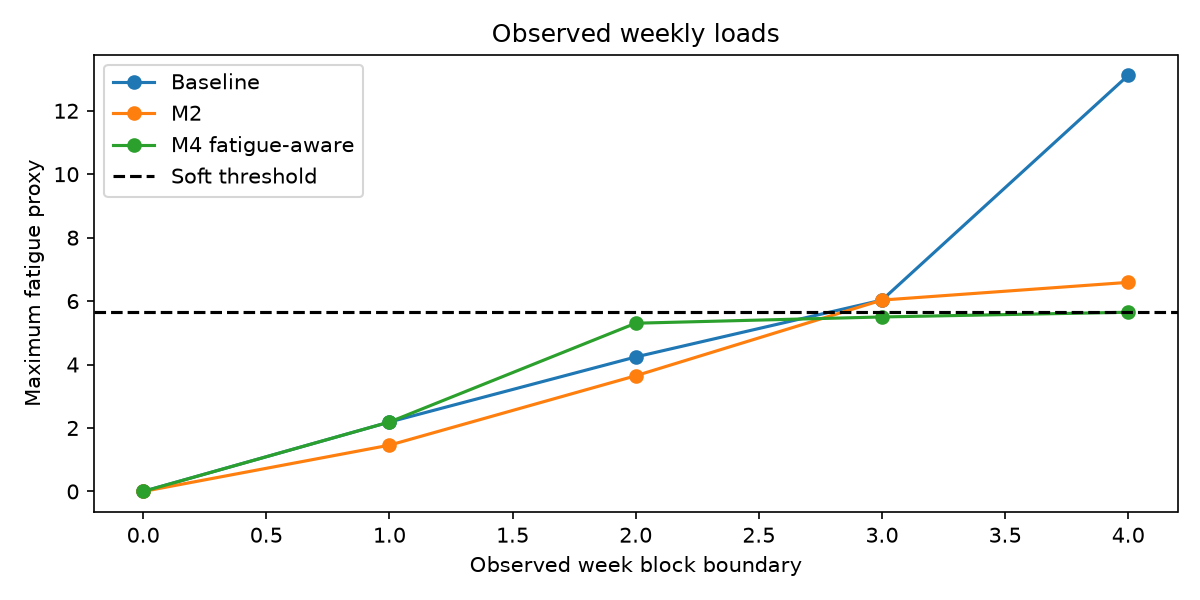
\includegraphics[width=0.78\textwidth]{figures/observed_fatigue.png}
\caption{Mức fatigue cực đại qua $4$ khối tuần lịch sử: M4 Fatigue-Aware giữ toàn bộ quỹ đạo dưới ngưỡng mềm $H = 5{,}660$ (tổng vượt ngưỡng $= 0{,}000$), giữ nguyên $\text{max\_load} = 11$ và $L_1 = 36{,}329$.}
\label{fig:m4_obs}
\end{figure}

\begin{figure}[htbp]
\centering
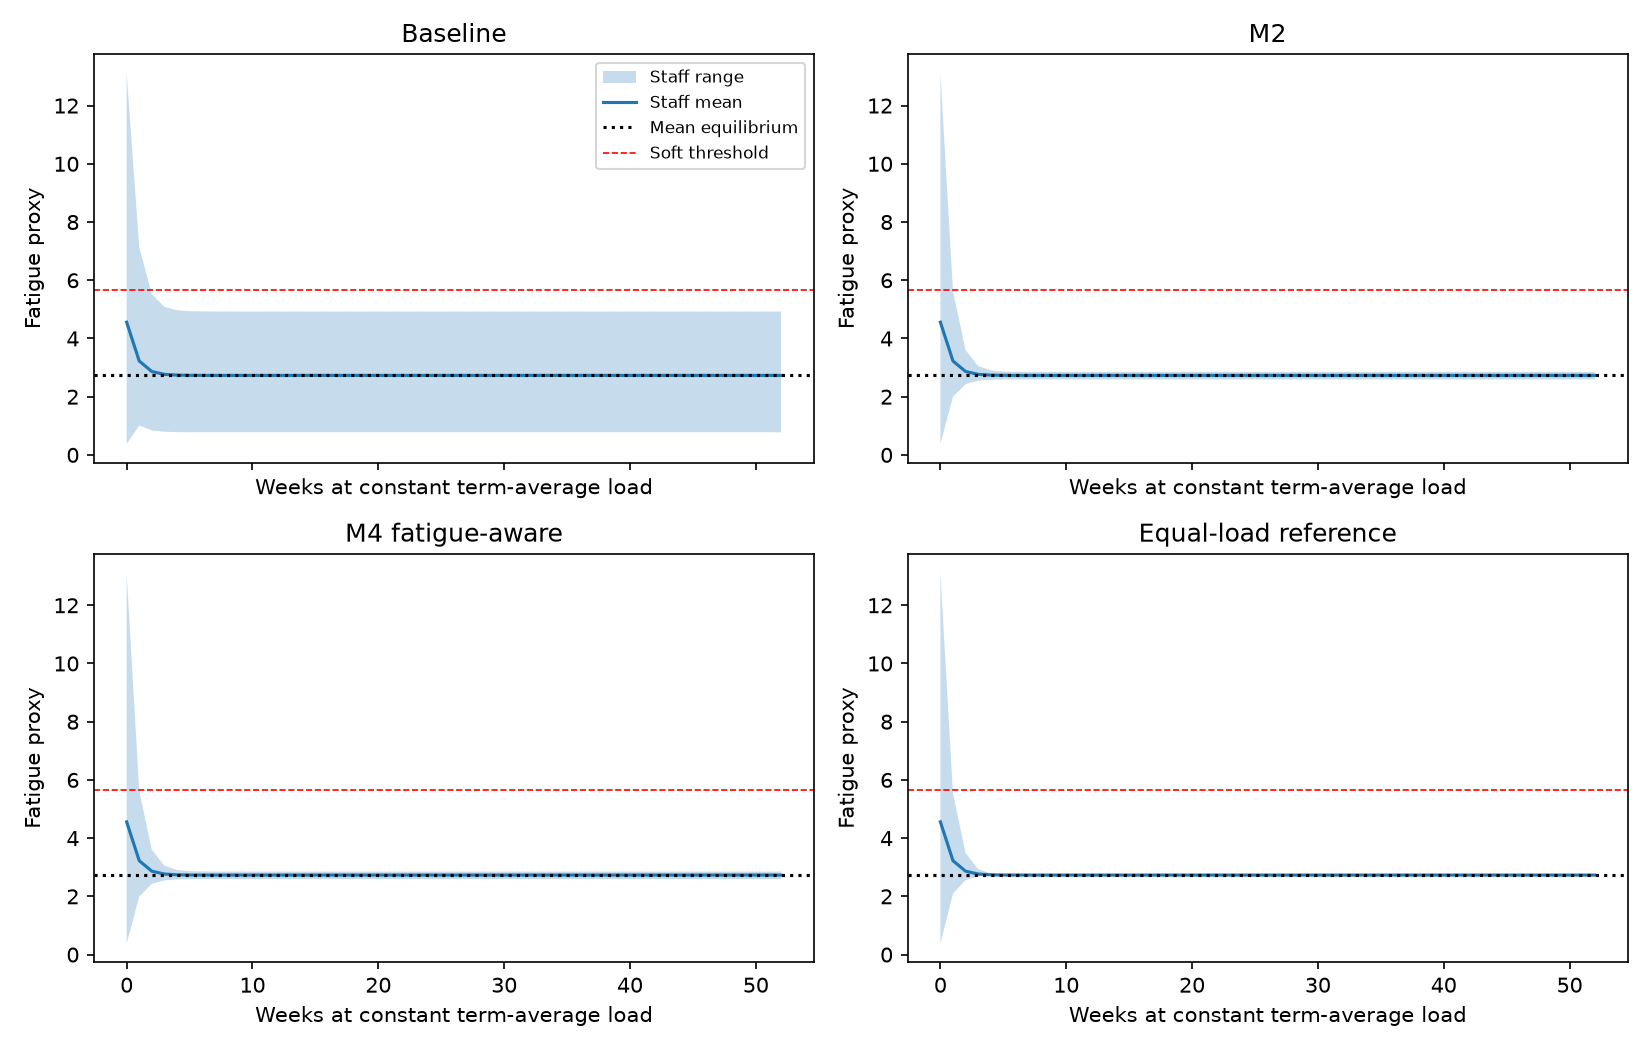
\includegraphics[width=0.86\textwidth]{figures/fatigue_equilibrium.png}
\caption{Quỹ đạo hội tụ $52$ tuần (dải $\min$--$\max$ và trung bình) dưới tải hằng kỳ đối với $4$ kịch bản, bắt đầu từ trạng thái cuối không đồng đều của Baseline.}
\label{fig:m4_eq}
\end{figure}

\begin{figure}[htbp]
\centering
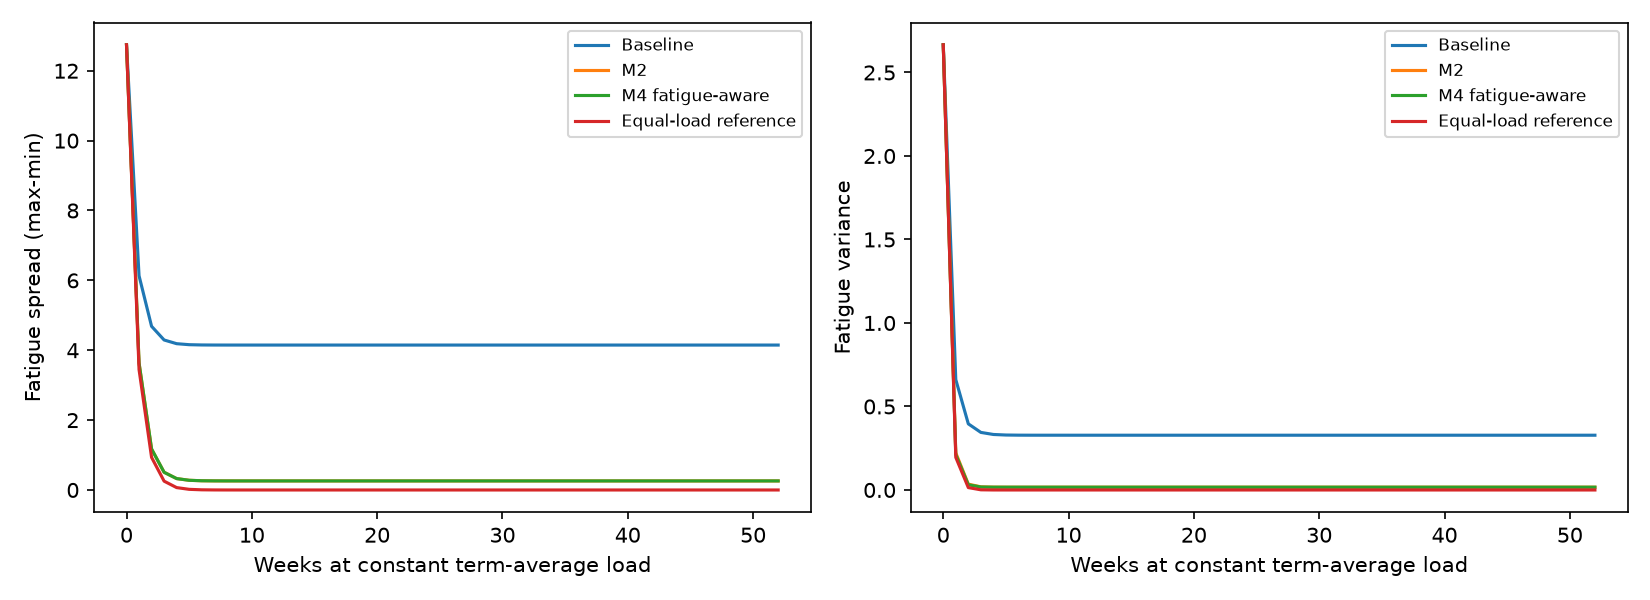
\includegraphics[width=0.86\textwidth]{figures/fairness.png}
\caption{Sự co hẹp theo hàm mũ của độ trải ($\operatorname{spread}$) và phương sai ($\operatorname{Var}$) fatigue theo thời gian, chứng minh tính chất hút công bằng của điểm cân bằng.}
\label{fig:m4_fair}
\end{figure}
\FloatBarrier
\newpage

\section{Module 5: Tích hợp Hệ thống và Ứng dụng Web Streamlit}
\label{sec:m5}

\subsection{Kiến trúc Mô-đun và Tối ưu Trải nghiệm Thuyết trình}
Để đưa toàn bộ chuỗi mô hình hóa từ chứng minh logic đến hoạch định dài hạn tới tay người điều phối thi, Module 5 xây dựng ứng dụng web \textbf{Streamlit} tại \texttt{app/app.py} với thiết kế tách biệt hoàn toàn lớp giao diện khỏi lõi thuật toán của Modules 1--4:
\begin{itemize}
    \item \textbf{Lớp điều phối và giao diện (\texttt{app.py}, \texttt{presentation.py}, \texttt{presentation.css}, \texttt{presentation\_\allowbreak views.py}, \texttt{theory\_\allowbreak content.py}):} Thiết lập thanh điều hướng $6$ chặng tương ứng mạch bài toán (\textit{Tổng quan}, \textit{1 · Logic}, \textit{2 · Xếp lịch}, \textit{3 · DFA}, \textit{4 · Fatigue}, \textit{Demo đầu-cuối}) cùng nút chuyển slide \textit{Phần trước / Phần tiếp}, các thẻ tổng hợp lý thuyết đối chiếu trực tiếp slide CO2011 và bảng kiểm tra quy mô.
    \item \textbf{Lớp Adapter đọc/gọi Modules 1--4 (\texttt{data\_\allowbreak views.py}, \texttt{solver\_\allowbreak views.py}, \texttt{temporal\_\allowbreak views.py}, \texttt{dynamics\_\allowbreak views.py}):} Gọi trực tiếp các hàm lõi (\texttt{encode\_\allowbreak invigilator\_\allowbreak assignment}, \texttt{solve\_\allowbreak instance}, \texttt{extract\_\allowbreak minimal\_\allowbreak core}, \texttt{build\_\allowbreak model}, \texttt{solve}, \texttt{check\_\allowbreak schedule}, \texttt{DFA.accepts}, \texttt{add\_\allowbreak regular\_\allowbreak constraint}, \texttt{calibrate}, \texttt{simulate}) mà không sửa đổi mã nguồn các module trước.
    \item \textbf{Tối ưu hiệu năng và kiểm soát an toàn (\texttt{precompute.py}, \texttt{m5\_\allowbreak bundle.json}):} Kết quả nặng trên toàn bộ dữ liệu ($73 \times 83$) được tính sẵn ngoại tuyến qua \texttt{python -m app.precompute} kèm mã băm SHA-256 kiểm chứng dữ liệu và seed; các lát cắt tương tác (\textit{Toy}, \textit{M1 Slice}, \textit{1 tuần}, \textit{2 tuần}) chạy giải trực tiếp trong phiên với bộ nhớ đệm \texttt{@st.cache\_\allowbreak data} và giới hạn thời gian CBC tùy chỉnh ($5$--$120\text{ s}$). Tệp CSV tải lên được kiểm tra chặt giới hạn an toàn ($\le 512\text{ KiB}$, $\le 2{,}000$ dòng, $\le 150$ người/ca, $\le 120$ ngày lịch).
\end{itemize}

\subsection{Đối chiếu Kết quả Đầu-Cuối trên Toàn bộ Dữ liệu}
Bảng~\ref{tab:e2e_summary} tổng hợp toàn bộ chỉ số của bốn phương án phân công trên cùng dữ liệu thực và cùng \texttt{seed = 1358677812} (trích từ \texttt{app/\allowbreak m5\_\allowbreak bundle.json}), cho thấy sự bổ trợ tất yếu giữa bốn học phần:

\begin{table}[htbp]
\centering
\caption{Bảng đối chiếu đầu-cuối (M1--M4) cho $4$ lịch phân công trên toàn bộ $73$ cán bộ và $83$ ca thi.}
\label{tab:e2e_summary}
\footnotesize
\setlength{\tabcolsep}{3.5pt}
\renewcommand{\arraystretch}{1.22}
\begin{tabularx}{\textwidth}{@{} L r r r r r r c r r @{}}
\toprule
\textbf{Phương án} & \textbf{Hard} & \textbf{Max} & \textbf{Spread} & \textbf{$L_1$} & \textbf{LOC} & \textbf{Obj} & \makecell[bc]{\textbf{DFA}\\\textbf{đạt}} & \makecell[br]{\textbf{Eq.}\\\textbf{Spread}} & \makecell[br]{\textbf{Vượt}\\\textbf{$H$}} \\
\midrule
Baseline & $0$ & $19$ & $16$ & $115{,}397$ & $162$ & $264{,}777$ & $41/73$ & $4{,}148$ & $16{,}312$ \\
M2 Optimal & $0$ & $11$ & $1$ & $36{,}329$ & $28$ & $59{,}849$ & $24/73$ & $0{,}259$ & $3{,}287$ \\
M2 + R1$\times$R2$\times$R3 & $0$ & $11$ & $1$ & $36{,}329$ & $36$ & $66{,}569$ & $\mathbf{73/73}$ & $0{,}259$ & $1{,}914$ \\
M4 Fatigue-Aware & $0$ & $11$ & $1$ & $36{,}329$ & $28$ & $59{,}849$ & $24/73$ & $0{,}259$ & $\mathbf{0{,}000}$ \\
\bottomrule
\end{tabularx}
\end{table}

\begin{notebox}{Thông điệp tích hợp cốt lõi từ Module 5}
\begin{enumerate}
    \item \textbf{Tính khả thi (M1) $\neq$ Tối ưu công bằng (M2):} Lịch \texttt{Baseline} hợp lệ mọi ràng buộc cứng H1--H3 nhưng tải đỉnh lên tới $19$ và $L_1 = 115{,}397$; M2 hạ tải đỉnh xuống chặn dưới $t^* = 11$ và giảm $L_1$ gần $3{,}2\times$.
    \item \textbf{Công bằng tổng (M2) $\neq$ Hợp lệ theo thời gian (M3):} Lịch \texttt{M2 Optimal} dù tối ưu tổng ca nhưng khiến $49/73$ cán bộ vi phạm các quy tắc nghỉ ngơi R1--R3; tích hợp flow DFA đưa tỷ lệ đạt chuẩn lên $73/73$ mà không làm tăng tải đỉnh $11$.
    \item \textbf{Công bằng tĩnh $\neq$ An toàn quá độ (M4):} \texttt{M4 Fatigue-Aware} giữ nguyên $t^*=11, L_1=36{,}329$ như M2 nhưng tái phân bổ nhịp độ giữa các tuần để xóa sạch phần vượt ngưỡng mệt mỏi $H = 5{,}660$ ($16{,}312 \to 3{,}287 \to 0{,}000$).
\end{enumerate}
\end{notebox}

\subsection{Khả năng Tái lập và Kiểm thử Hệ thống}
Toàn bộ kết quả trên được tái lập từ mã nguồn sạch qua:
\begin{itemize}
    \item \texttt{python run\_all.py --seed \$(cat data/seed.txt)}: chạy tuần tự M1--M5 và kiểm chứng các bất biến toán học.
    \item \texttt{streamlit run app/app.py}: khởi chạy giao diện trình chiếu tương tác trực tiếp.
    \item Bộ kiểm thử tự động \texttt{pytest} bao phủ toàn bộ quy trình (kiểm thử đơn vị CNF, cầu nối Logic-LP, mô hình ILP, bộ kiểm định độc lập, DFA R1--R4, tối giản, flow brute-force, hệ động lực Hướng B và tích hợp Streamlit).
\end{itemize}
\section{Kết luận và Hướng Phát triển}
\label{sec:conclusion}

\subsection{Tổng kết Kết quả Đạt được}
Đồ án đã hoàn thành việc xây dựng một hệ thống mô hình hóa toán học hoàn chỉnh, liên thông năm module cho bài toán phân công cán bộ coi thi tại CSE--HCMUT:
\begin{itemize}
    \item \textbf{Module 1 (Logic \& SAT):} Đặc tả đầy đủ H1--H3 bằng logic vị từ bậc nhất, mã hóa CNF bằng mạch đếm tuần tự tránh bùng nổ tổ hợp ($156{,}428$ mệnh đề trên dữ liệu thực), trích xuất chính xác Minimal UNSAT Core ($6$ ràng buộc) và kiểm chứng cầu nối sang 0/1 tuyến tính kèm $5$ phản chứng.
    \item \textbf{Module 2 (ILP):} Thiết lập mô hình biến thưa ($|A|=2{,}593$), tối ưu từ điển hai giai đoạn với dây cung \texttt{DEVC} đóng kín độ hở LP tại nút gốc ($0{,}17\text{ s}$), giảm tải đỉnh từ $19$ xuống mức tối ưu lý thuyết $11$, kiểm định bởi bộ validator độc lập và chứng minh sai lầm của việc bỏ H2 hoặc thư giãn liên tục.
    \item \textbf{Module 3 (Automata):} Mô hình hóa chuỗi ngày làm việc $\Sigma^{27}$, tối giản tích $R_1 \times R_2 \times R_3$ từ $259$ xuống $15$ trạng thái, phân rã đồ thị phân tầng flow ILP đạt $73/73$ cán bộ hợp lệ, đồng thời chứng minh chặt chẽ ranh giới giữa ngôn ngữ chính quy R4 và ngôn ngữ phi chính quy $\#_M = \#_A$.
    \item \textbf{Module 4 (Discrete Dynamics):} Hiệu chuẩn mô hình vector fatigue Hướng B ($a = 0{,}270634$, $\rho(J) < 1$), chứng minh sự hội tụ về công bằng ($\operatorname{spread} \to 0$) và đưa ngưỡng mềm $H = 5{,}660$ vào ILP để đưa mức vượt ngưỡng về $0{,}000$.
    \item \textbf{Module 5 (Web App):} Tích hợp toàn diện bốn module lên nền tảng Streamlit trực quan, nhẹ và sẵn sàng thuyết trình.
\end{itemize}

\subsection{Hạn chế và Hướng Mở rộng}
Nhóm thẳng thắn ghi nhận bốn hạn chế của mô hình hiện tại: (1) lịch khả dụng và nguyện vọng cơ sở là dữ liệu giả lập từ seed thay cho khảo sát thực tế; (2) phép nén $1$ ký hiệu/ngày theo ưu tiên $\texttt{N} > \texttt{A} > \texttt{M}$ khiến các ngày $2$ ca (\texttt{M+A}) nghiêng về \texttt{A} khi đếm R4; (3) hệ số $a$ hồi quy từ suất tuần lịch sử có $R^2 = 0{,}0619$ do phân bố ca thi không đều giữa các tuần và chưa phản ánh mệt mỏi sinh lý thực; (4) do ràng buộc thời gian giải ($150\text{ s}$), phương án \texttt{M4 Fatigue-Aware} được giải tách riêng với ràng buộc flow M3 và chưa đưa R4 ($99$ trạng thái) vào flow ILP. Trong tương lai, hệ thống có thể mở rộng bằng cách kết hợp đồng thời flow M3 và ngưỡng $H$ của M4 trong một mô hình ILP thống nhất (biểu diễn R4 bằng $2T$ ràng buộc tuyến tính thay cho trạng thái ô-tô-mát) và nâng cấp lên mô hình tầm cuốn chiếu phản hồi vòng kín (Hướng A) khi có dữ liệu nghỉ phép thực tế.

\begin{thebibliography}{99}
\small
\bibitem{slides_logic} M. V. M. Nguyen, K. A. Nguyen et al., \textit{CO2011 Lecture Slides: Chapter 1 -- Logic Theory and Program Verification}, CSE--HCMUT, 2021--2026.
\bibitem{slides_ilp} M. V. M. Nguyen, K. A. Nguyen et al., \textit{CO2011 Lecture Slides: Chapter 3 -- Integer Optimization: Models and Practical Usages}, CSE--HCMUT, 2021--2026.
\bibitem{slides_automata} T. V. Hoai, H. T. Nguyen, N. A. Khuong, L. H. Trang, \textit{CO2011 Lecture Slides: Chapter 4 -- Automata and Formal Languages}, CSE--HCMUT, 2021--2026.
\bibitem{slides_dynamics} N. A. Khuong, H. T. Nguyen, M. V. M. Nguyen, \textit{CO2011 Lecture Slides: Chapter 5/6 -- Dynamical Systems}, CSE--HCMUT, 2021--2026.
\bibitem{hanum2015} F. Hanum, M. A. Romliyah, T. Bakhtiar, ``Exam invigilators assignment problem: a goal programming approach,'' \textit{Applied Mathematical Sciences}, 9(58):2871--2880, 2015.
\bibitem{burke2004} E. K. Burke et al., ``The state of the art of nurse rostering,'' \textit{Journal of Scheduling}, 7(6):441--499, 2004.
\bibitem{pesant2004} G. Pesant, ``A regular language membership constraint for finite sequences of variables,'' in \textit{CP 2004}, LNCS 3258, pp. 482--495, Springer, 2004.
\bibitem{cote2011} M.-C. C\^{o}t\'{e}, B. Gendron, L.-M. Rousseau, ``Grammar-based integer programming models for multiactivity shift scheduling,'' \textit{Management Science}, 57(1):151--163, 2011.
\bibitem{sinz2005} C. Sinz, ``Towards an optimal CNF encoding of boolean cardinality constraints,'' in \textit{CP 2005}, LNCS 3709, pp. 827--831, Springer, 2005.
\bibitem{rosen2019} K. H. Rosen, \textit{Discrete Mathematics and Its Applications}, 8th ed., McGraw-Hill, 2019.
\bibitem{huth2004} M. Huth, M. Ryan, \textit{Logic in Computer Science}, 2nd ed., Cambridge University Press, 2004.
\bibitem{linz2017} P. Linz, \textit{An Introduction to Formal Languages and Automata}, 6th ed., Jones \& Bartlett, 2017.
\bibitem{hopcroft2006} J. E. Hopcroft, R. Motwani, J. D. Ullman, \textit{Introduction to Automata Theory, Languages, and Computation}, 3rd ed., Pearson, 2006.
\bibitem{matousek2007} J. Matou\v{s}ek, B. G\"{a}rtner, \textit{Understanding and Using Linear Programming}, Springer, 2007.
\bibitem{nemhauser1999} G. L. Nemhauser, L. A. Wolsey, \textit{Integer and Combinatorial Optimization}, Wiley, 1999.
\bibitem{giordano2013} F. R. Giordano, W. P. Fox, S. B. Horton, \textit{A First Course in Mathematical Modeling}, 5th ed., Cengage, 2013.
\bibitem{elaydi2005} S. Elaydi, \textit{An Introduction to Difference Equations}, 3rd ed., Springer, 2005.
\end{thebibliography}

% ==================== PHỤ LỤC ====================
\newpage
\appendix
\section{Phụ lục A: Chứng minh Toán học Chi tiết}

\subsection{Chứng minh Bổ đề Bơm cho Cân bằng Chính xác \texorpdfstring{$L_= = \{w \in \Sigma^* : \#_M(w) = \#_A(w)\}$}{L= = \{w in Sigma* : \#M(w) = \#A(w)\}}}
\label{app:pumping}
\begin{proof}
Giả sử phản chứng rằng $L_= = \{w \in \Sigma^* : \#_M(w) = \#_A(w)\}$ là một ngôn ngữ chính quy trên $\Sigma = \{\texttt{M}, \texttt{A}, \texttt{N}, \texttt{-}\}$. Xét ngôn ngữ $R = \texttt{M}^*\texttt{A}^*$; rõ ràng $R$ chính quy vì được biểu diễn trực tiếp bởi biểu thức chính quy. Do lớp ngôn ngữ chính quy đóng dưới phép giao, ngôn ngữ:
\begin{equation*}
    L' = L_= \cap R = \{\texttt{M}^n \texttt{A}^n : n \ge 0\}
\end{equation*}
cũng phải là ngôn ngữ chính quy. Theo Bổ đề Bơm cho ngôn ngữ chính quy, tồn tại số nguyên dương $p \ge 1$ (độ dài bơm) sao cho mọi từ $s \in L'$ có $|s| \ge p$ đều phân tích được thành $s = xyz$ thỏa mãn đồng thời ba điều kiện: (i) $|xy| \le p$, (ii) $|y| \ge 1$, và (iii) $\forall i \ge 0, \; xy^i z \in L'$.

Chọn từ $s = \texttt{M}^p \texttt{A}^p \in L'$ có độ dài $|s| = 2p \ge p$. Vì $|xy| \le p$, cả hai tiền tố $x$ và $y$ đều nằm trọn trong khối $p$ ký hiệu $\texttt{M}$ đầu tiên. Do $|y| \ge 1$, tồn tại số nguyên $k$ với $1 \le k \le p$ sao cho $y = \texttt{M}^k$. Lấy $i = 0$, ta thu được từ mới:
\begin{equation*}
    x y^0 z = xz = \texttt{M}^{p-k} \texttt{A}^p.
\end{equation*}
Khi đó $\#_M(xz) = p - k < p = \#_A(xz)$ (do $k \ge 1$), suy ra $xz \notin L'$, mâu thuẫn với điều kiện (iii). (Ví dụ minh họa với $p = 3$, $s = \texttt{MMMAAA}$, tách $x=\varepsilon, y=\texttt{M}$ cho $xz = \texttt{MMAAA} \notin L'$). Vậy $L'$ không chính quy, kéo theo $L_=$ không chính quy. Lưu ý: trên một độ dài hữu hạn cố định $T$, tập từ dài $T$ có $\#_M = \#_A$ là hữu hạn nên chính quy, nhưng DFA tối thiểu đòi hỏi $O(T)$ trạng thái phụ thuộc vào $T$, trong khi R4 ($|\#_M - \#_A| \le c$) chỉ cần $2c+2$ trạng thái cố định.
\end{proof}

\subsection{Chứng minh Tính Tương đương của Ràng buộc Luồng Regular-to-ILP}
\label{app:flow_proof}
\begin{proof}
Cho DFA hoàn chỉnh $\mathcal{A} = (Q, \Sigma, q_0, \delta, F)$ và chuỗi nhị phân ngày $s_{t, a} \in \{0, 1\}$ ($\sum_a s_{t, a} = 1$ tại mỗi $t = 0, \dots, T-1$) xác định duy nhất một từ $w = w_1\dots w_T$ với $s_{t, w_{t+1}} = 1$. Giả sử hệ phương trình \texttt{SRC}, \texttt{FLOW}, \texttt{LINK} có nghiệm $y_{t, q, a} \in [0, 1]$. Ta chứng minh bằng quy nạp theo $t$ rằng toàn bộ $1$ đơn vị luồng tại tầng $t$ nằm trọn tại đúng đỉnh $q_t = \hat{\delta}(q_0, w_1\dots w_t)$:
\begin{itemize}
    \item \textit{Bước cơ sở ($t = 0$):} Phương trình \texttt{SRC} đặt $\sum_a y_{0, q_0, a} = 1$, và không có đỉnh nào khác ở tầng $0$ có luồng ra.
    \item \textit{Bước quy nạp ($t \to t+1$):} Theo giả thiết quy nạp, tổng luồng tại tầng $t$ dồn ở $q_t$. Theo phương trình \texttt{LINK}, $\sum_q y_{t, q, a} = s_{t, a} = 0$ với mọi $a \neq w_{t+1}$ và $y \ge 0$, nên mọi cung có nhãn $a \neq w_{t+1}$ đều mang luồng $0$. Do đó toàn bộ $1$ đơn vị luồng từ $(t, q_t)$ phải đi theo duy nhất cung nhãn $w_{t+1}$ tới đỉnh $(t+1, \delta(q_t, w_{t+1})) = (t+1, q_{t+1})$.
\end{itemize}
Tại tầng cuối $T$, vì đồ thị phân tầng chỉ tạo biến $y$ trên các cung dẫn tới $F$, việc tồn tại luồng $1$ đơn vị tới tầng $T$ tương đương $q_T \in F$, tức $w \in L(\mathcal{A})$. Hơn nữa, chứng minh chỉ dùng tính nhị phân của $s_{t,a}$ nên $y_{t,q,a}$ giữ nguyên dạng liên tục $[0,1]$ mà vẫn tự động nhận giá trị $0/1$.
\end{proof}

\subsection{Chứng minh Co hẹp Độ trải và Phương sai trong Hệ Động lực Hướng B}
\label{app:dynamics_proof}
Với hệ $F_{n+1} = a F_n + b \ell - r \rho$, khi mọi cán bộ có chung tải tuần $\ell_i = \mu$ và nghỉ $\rho_i = \bar{\rho}$, ta có điểm cân bằng chung $F^* = \frac{b\mu - r\bar{\rho}}{1-a}$ cho mọi thành phần. Lấy hiệu giữa hai cán bộ $i, j$ bất kỳ:
\begin{equation*}
    F_{n+1, i} - F_{n+1, j} = a(F_{n, i} - F_{n, j}) \implies F_{n, i} - F_{n, j} = a^n (F_{0, i} - F_{0, j}).
\end{equation*}
Do đó $\operatorname{spread}(F_n) = \max_{i,j} |F_{n,i} - F_{n,j}| = |a|^n \operatorname{spread}(F_0)$ và tương tự $F_{n, i} - \bar{F}_n = a^n (F_{0, i} - \bar{F}_0)$ dẫn tới $\operatorname{Var}(F_n) = a^{2n} \operatorname{Var}(F_0)$. Khi $|a| < 1$, cả $\operatorname{spread}(F_n)$ và $\operatorname{Var}(F_n)$ đều hội tụ về $0$ theo hàm mũ.

\section{Phụ lục B: Kết quả Kiểm chứng Tự động}

\subsection{Kiểm chứng Vét cạn Mô hình Luồng Regular-to-ILP (\texorpdfstring{$T = 7$}{T = 7})}
Trong \texttt{m3\_\allowbreak automata/\allowbreak regular\_\allowbreak to\_\allowbreak ilp.py}, hàm \texttt{brute\_\allowbreak force\_\allowbreak check()} đối chiếu giá trị tối ưu của mô hình luồng ILP với phương pháp duyệt vét cạn toàn bộ $4^7 = 16{,}384$ chuỗi trên $16$ kịch bản kiểm thử ($4$ ô-tô-mát R1, R2, R3, $R_1\times R_2\times R_3$ $\times$ $2$ hàm mục tiêu \texttt{random}/\texttt{max\_work} $\times$ $2$ chế độ cố định ngày): toàn bộ $\mathbf{16/16}$ trường hợp khớp tuyệt đối (Bảng~\ref{tab:app_bf}, trích từ \texttt{extra/\allowbreak regular\_\allowbreak to\_\allowbreak ilp.json}).

\begin{table}[htbp]
\centering
\caption{Kết quả đối chiếu $16/16$ kịch bản vét cạn trên khung $T=7$ ngày của \texttt{regular\_to\_ilp.py}.}
\label{tab:app_bf}
\footnotesize
\setlength{\tabcolsep}{6pt}
\renewcommand{\arraystretch}{1.16}
\begin{tabularx}{\textwidth}{@{} c L c r r c @{}}
\toprule
\textbf{DFA} & \textbf{Hàm mục tiêu} & \textbf{Cố định ngày} & \textbf{Brute-force} & \textbf{Flow ILP} & \textbf{Chuỗi tối ưu} \\
\midrule
R1 & \texttt{random}    & Không & $-16{,}00$ & $-16{,}00$ & \texttt{--AN--N} \\
R1 & \texttt{random}    & Có    & $-11{,}00$ & $-11{,}00$ & \texttt{MN--MM-} \\
R1 & \texttt{max\_work} & Không & $-6{,}25$  & $-6{,}25$  & \texttt{N-NN-NN} \\
R1 & \texttt{max\_work} & Có    & $-6{,}00$  & $-6{,}00$  & \texttt{NN-NM-N} \\
\addlinespace[3pt]
R2 & \texttt{random}    & Không & $-14{,}00$ & $-14{,}00$ & \texttt{AMN-N-A} \\
R2 & \texttt{random}    & Có    & $-20{,}00$ & $-20{,}00$ & \texttt{MMAMAN-} \\
R2 & \texttt{max\_work} & Không & $-7{,}25$  & $-7{,}25$  & \texttt{MMMMAMN} \\
R2 & \texttt{max\_work} & Có    & $-6{,}50$  & $-6{,}50$  & \texttt{MN-MMMN} \\
\addlinespace[3pt]
R3 & \texttt{random}    & Không & $-24{,}00$ & $-24{,}00$ & \texttt{-MM---A} \\
R3 & \texttt{random}    & Có    & $-21{,}00$ & $-21{,}00$ & \texttt{--M-ANN} \\
R3 & \texttt{max\_work} & Không & $-5{,}00$  & $-5{,}00$  & \texttt{-N--NNN} \\
R3 & \texttt{max\_work} & Có    & $-5{,}00$  & $-5{,}00$  & \texttt{-NNNN--} \\
\addlinespace[3pt]
Prod & \texttt{random}    & Không & $-29{,}00$ & $-29{,}00$ & \texttt{N--MA-A} \\
Prod & \texttt{random}    & Có    & $-18{,}00$ & $-18{,}00$ & \texttt{-N-MA-A} \\
Prod & \texttt{max\_work} & Không & $-5{,}00$  & $-5{,}00$  & \texttt{N-N-N-N} \\
Prod & \texttt{max\_work} & Có    & $-4{,}75$  & $-4{,}75$  & \texttt{N-AN--N} \\
\bottomrule
\end{tabularx}
\end{table}

\section{Phụ lục C: Phân công Đóng góp và Khai báo Sử dụng AI}

\subsection[Bảng Phân công Nhiệm vụ Chính theo Module]{Bảng Phân công Nhiệm vụ Chính theo Module\protect\\(trích {\normalfont\ttfamily CONTRIBUTIONS.md})}
Mỗi thành viên đều tham gia đóng góp mã nguồn và kiểm tra chéo trên cả $4$ module lý thuyết với tỷ lệ hoàn thành phân công $100\%$:

\begin{table}[htbp]
\centering
\caption{Tóm tắt phân công phụ trách chính của $5$ thành viên trong nhóm \texttt{CO2011-261-A01-2551896}.}
\label{tab:app_contrib}
\footnotesize
\setlength{\tabcolsep}{5pt}
\renewcommand{\arraystretch}{1.22}
\begin{tabularx}{\textwidth}{@{} l L @{}}
\toprule
\textbf{Thành viên (MSSV)} & \textbf{Hạng mục phụ trách chính (Primary Ownership)} \\
\midrule
2551922 Chu Ngọc Phúc Thành & M1: Đặc tả vị từ (1.1); M2: Ràng buộc cứng H1--H3, Validator độc lập (2.4) \& Phản ví dụ (2.10); M3: R4 \& Bổ đề Bơm (3.4); M4: Mô hình vector mệt mỏi (\texttt{fatigue.py}). \\
2551919 Đặng Nguyễn Thiên Phúc & M1: Ánh xạ biến \& mã hóa CNF (1.2); M2: Hàm mục tiêu (2.3) \& Hiệu năng (2.9); M3: Mã hóa chuỗi, lớp DFA \& tích hợp M3 (3.1); M4: Ngưỡng mềm ILP (\texttt{planning.py}). \\
2551913 Võ Nguyễn Vĩ Nguyên & M1: Giải SAT \& Minimal UNSAT Core (1.2); M2: Phạt mềm (2.5) \& Độ nhạy/Hiệu chỉnh (2.8); M3: Tích \& Tối giản (3.2); M4: Tài liệu kỹ thuật. \\
2551931 Đinh Hoàng Quang Vinh & M1: Tiền xử lý lát cắt (1.2); M2: Tập hợp, biến thưa \& dữ liệu giả lập (2.1, 2.2, 2.6); M3: DFA R1--R3 (3.1); M4: Pipeline \& đồ thị (\texttt{run.py}, \texttt{plots.py}). \\
2551896 Nguyễn Quốc Hùng & M1: Cầu nối Logic-to-LP (1.3); M2: Lắp ráp mô hình, bộ giải CBC \& \texttt{run\_all.py} (2.7); M3: Flow ILP (3.3); M4: Trích xuất tải tuần (\texttt{workload.py}). \\
\bottomrule
\end{tabularx}
\end{table}

\subsection{Khai báo Sử dụng Công cụ AI (AI-Use Declaration)}
Tuân thủ quy định minh bạch học thuật của môn học (\texttt{README.md}), nhóm sử dụng trợ lý AI như công cụ hỗ trợ kỹ thuật để: (i) thảo luận thiết kế bộ mã hóa CNF và cầu nối Logic-to-LP ở Module 1; (ii) hỗ trợ rà soát cú pháp PuLP, sinh kiểm thử đối chiếu ở Module 2; (iii) đề xuất cấu trúc JSON cho DFA và quy tắc ưu tiên $\texttt{N} > \texttt{A} > \texttt{M}$ (đã được giảng viên xác nhận trên diễn đàn ngày 21/10/2026) ở Module 3; (iv) hỗ trợ cài đặt kiểm thử số, vẽ biểu đồ ở Module 4; (v) thiết kế lại giao diện trình chiếu Streamlit ở Module 5 và rà soát trình bày báo cáo LaTeX. Mọi mô hình toán học, mã nguồn và số liệu thực nghiệm đều do các thành viên trực tiếp kiểm tra, hiểu rõ và xác nhận qua bộ kiểm thử tự động.

\end{document}